\pdfoutput=1
\documentclass[11pt]{article}

\usepackage[letterpaper,margin=1in]{geometry}
\usepackage[T1]{fontenc}
\usepackage[utf8]{inputenc}
\usepackage{lmodern}
\usepackage{amsmath,amssymb,amsthm,mathtools}
\usepackage{bm}
\usepackage{microtype}
\usepackage{booktabs}
\usepackage{graphicx}
\usepackage{placeins}
\usepackage{tikz}
\usetikzlibrary{arrows.meta}
\usepackage{caption}
\usepackage{enumitem}
\usepackage[round,authoryear]{natbib}
\usepackage{xcolor}
\usepackage{hyperref}
\usepackage[nameinlink,noabbrev]{cleveref}

\hypersetup{
  colorlinks=true,
  linkcolor=blue!45!black,
  citecolor=blue!45!black,
  urlcolor=blue!45!black,
  pdftitle={Exact Sparsity without Penalization: Randomly Reweighted NPMLEs
    for Gaussian Mixtures},
  pdfauthor={Hansheng Jiang}
}
% Placeholder: the public Lean repository has not been created yet.
\newcommand{\leanrepo}{\url{https://github.com/hanshengjiang/sparse-npmle-lean}}
\renewcommand{\baselinestretch}{1.05}
\setlength{\parskip}{0.3em}
\setlength{\parindent}{15pt}
\setlist[itemize]{leftmargin=1.4em,itemsep=0.15em,topsep=0.3em}
\setlist[enumerate]{leftmargin=1.7em,itemsep=0.15em,topsep=0.3em}
\allowdisplaybreaks[2]
\setlength{\emergencystretch}{1.5em}

\newtheorem{theorem}{Theorem}
\newtheorem{proposition}{Proposition}
\newtheorem{lemma}{Lemma}
\newtheorem{corollary}{Corollary}
\theoremstyle{definition}
\newtheorem{definition}{Definition}
\newtheorem{assumption}{Assumption}
\theoremstyle{remark}
\newtheorem{remark}{Remark}

\DeclareMathOperator*{\argmax}{arg\,max}
\DeclareMathOperator*{\argmin}{arg\,min}
\DeclareMathOperator{\conv}{conv}
\DeclareMathOperator{\supp}{supp}
\DeclareMathOperator{\rank}{rank}
\DeclareMathOperator{\diag}{diag}
\DeclareMathOperator{\KL}{KL}
\DeclareMathOperator{\TV}{TV}
\newcommand{\Pcal}{\mathcal P}
\newcommand{\Mcal}{\mathcal M}
\newcommand{\Ccal}{\mathcal C}
\newcommand{\Acal}{\mathcal A}
\newcommand{\Ucal}{\mathcal U}
\newcommand{\Ncal}{\mathcal N}
\newcommand{\RR}{\mathbb R}
\newcommand{\EE}{\mathbb E}
\newcommand{\PP}{\mathbb P}
\newcommand{\one}{\bm 1}
\newcommand{\norm}[1]{\lVert #1\rVert}
\newcommand{\abs}[1]{\lvert #1\rvert}
\newcommand{\ip}[2]{\langle #1,#2\rangle}
\newcommand{\vhat}{\widehat v}
\newcommand{\Ghat}{\widehat G}
\newcommand{\Gtil}{\widetilde G}
\newcommand{\vtil}{\widetilde v}
\newcommand{\eps}{\varepsilon}
\newcommand{\sext}{s_{\mathrm{ext}}}

\title{\bfseries Exact Sparsity without Penalization:\\
Randomly Reweighted NPMLEs for Gaussian Mixtures}
\author{Hansheng Jiang\\[0.3em]
\small Rotman School of Management, University of Toronto\\
\small \href{mailto:hansheng.jiang@rotman.utoronto.ca}{\texttt{hansheng.jiang@rotman.utoronto.ca}}}
\date{September 2026}

\input{numerics_v3/results/manuscript_values.tex}

\begin{document}
\maketitle

\begin{abstract}
The nonparametric maximum likelihood estimator (NPMLE) of a Gaussian
location mixture maximizes the likelihood over all mixing distributions.
Although the problem is convex in the fitted density, the maximizing mixing
law can be nonunique, and the classical bound on its number of atoms grows
linearly with the sample size.  We show that a vanishingly small random
perturbation of the likelihood resolves both issues.  The estimator
maximizes a single weighted likelihood with independent Gamma weights whose
concentration grows with $n$; unlike the Bayesian bootstrap, one draw is used
as a point estimator.  With high probability, this randomly reweighted NPMLE
is unique, has polylogarithmically many atoms in any fixed dimension, loses
only a vanishing amount of ordinary log-likelihood, and attains a
near-parametric Hellinger rate for density estimation.  Exact sparsity is
thus obtained without a support penalty and without sacrificing statistical
accuracy.  In simulations in one and two dimensions, its estimated mean squared Hellinger risk
is within $\numAbstractRiskPercent\%$ of that of the ordinary NPMLE in every design.  The proof
rests on an effective-dimension principle for positive kernel mixtures:
low-dimensional variation of the fitted values controls the support of every
extreme optimizer.
\end{abstract}

\noindent\textbf{Keywords:} Bayesian bootstrap; Gaussian mixtures; Hellinger
distance; nonparametric maximum likelihood; random regularization; sparsity;
weighted likelihood.

\smallskip
\noindent\textbf{MSC2020 subject classifications:} Primary 62G07;
secondary 62G05, 62G20.

%======================================================================
\section{Introduction}\label{sec:introduction}

Let $X_1,\ldots,X_n\in\RR^d$ be observations from a Gaussian location
mixture.  For a mixing distribution $G$ and the standard Gaussian density
$\phi_d$, write
\[
  f_G(x)=\int \phi_d(x-\theta)\,dG(\theta).
\]
The Kiefer--Wolfowitz NPMLE \citep{kieferwolfowitz1956} maximizes
$\sum_i\log f_G(X_i)$ over a convex class of probability measures.  It is attractive precisely because it does
not specify the number of mixture components.  The same infinite-dimensional
formulation, however, leaves a structural question: how complicated must an
exact maximizing mixing law be?

Classical convex geometry guarantees the existence of a maximizer with at
most $n$ atoms, and all maximizers have the same fitted values at the sample
points; see \citet{lindsay1983geometry} and the subsequent mixture-likelihood
literature.  This deterministic $n$-point bound does not explain the much
smaller models often returned in practice.  In one dimension,
\citet{polyanskiywu2020} proved that the ordinary Gaussian-mixture NPMLE has
$O(\log n)$ atoms with high probability under sub-Gaussian sampling, a
phenomenon they called self-regularization.  In several dimensions,
quantitative polylogarithmic support control for the ordinary NPMLE remains
substantially more difficult.  Recent work of \citet{wang2026} establishes
qualitative finite support for every finite-data multivariate Gaussian NPMLE,
but does not give a polylogarithmic cardinality bound or generic uniqueness.

Beyond support size, Gaussian-mixture NPMLEs have been studied extensively as
estimators of mixing distributions, marginal densities, and empirical Bayes
rules; see, among others, \citet{laird1978}, \citet{koenkermizera2014},
\citet{zhang2009}, \citet{sahaguntuboyina2020}, and
\citet{soloffetal2025}.  The resulting density-estimation theory can be nearly
parametric up to logarithmic factors, and recent entropy characterizations
clarify the minimax benchmark \citep{jiaetal2023}.  These results establish the
statistical value of the NPMLE, but they do not provide a unique exact mixing
representation with polylogarithmic support in several dimensions.

This paper takes a different route.  Rather than forcing the equal-weight
NPMLE to reveal a sparse representation, we introduce an asymptotically
negligible random tilt of the likelihood and analyze the optimizer selected by
that tilt.  Given a concentration parameter $\alpha_n$, draw independently
\[
 W_i\sim\mathrm{Gamma}(\alpha_n,\alpha_n),
 \qquad i=1,\ldots,n,
\]
where shape and rate are both $\alpha_n$, and define
\begin{equation}\label{eq:rrnpmle-intro}
 \Ghat_W\in\argmax_{G\in\Pcal(K)}
       \sum_{i=1}^n W_i\log f_G(X_i).
\end{equation}
The weights have mean one and variance $1/\alpha_n$.  After normalization,
$(W_i/\sum_jW_j)_i$ is Dirichlet with common parameter $\alpha_n$.
Dirichlet-weighted likelihoods are classical in the Bayesian bootstrap of
\citet{rubin1981} and the weighted likelihood bootstrap of
\citet{newtonraftery1994}.  Their customary role is to generate a distribution
of bootstrap or approximate posterior draws.  Here a single, increasingly
concentrated draw is used as a point estimator.  The concentration is chosen
to expose a sparse extreme point while keeping the statistical criterion
asymptotically indistinguishable from ordinary likelihood.

The main result shows that this randomization acts as an exact regularizer.
For a fixed compact parameter set and fixed dimension, set
\[
 r_n=\left(\frac{\log n}{\log\log n}\right)^d,
 \qquad \bar r_n=r_n+\log n,
 \qquad \alpha_n=\bar r_n\log n.
\]
Then, with probability at least $1-Cn^{-b}$ for every fixed $b>0$, the
weighted optimizer is unique and has at most $O(\bar r_n)$ atoms.  Its total
ordinary log-likelihood loss is $O(1/\log n)$, and its fitted log-likelihood
vector is equally close to the ordinary one in squared Euclidean norm.  Its
mixture density has the same near-parametric Hellinger accuracy established
here for all one-unit near-maximizers:
\[
 H^2(f_{\Ghat_W},f_{G^*})
 =O_{\PP}\!\left(\frac{(\log n)^{d+1}}
 {n(\log\log n)^d}\right).
\]
The perturbation itself vanishes:
$\max_i\abs{W_i-1}=O_{\PP}(\bar r_n^{-1/2})$.  Moreover, for any prescribed
$L>0$, one may instead take $\alpha_n=n^{2L+2}$; the perturbation is then at
most $n^{-L}$ with overwhelming probability, yet the same exact support and
Hellinger conclusions continue to hold.

The contribution is therefore not random weighting per se.  It is the joint
estimator theorem: a single reweighted NPMLE is simultaneously
\emph{unique}, \emph{exactly sparse}, \emph{near-optimal in ordinary
likelihood}, and \emph{globally accurate in Hellinger distance}.  Randomness
resolves degeneracy, but the support theorem is not a generic tie-breaking
statement.  Its cardinality is controlled by an analytic effective dimension
of the Gaussian fitted-value set.

A numerical study makes the proximity statement operational.  Along a
regularization path, weight dispersion decays at the expected
$\alpha^{-1/2}$ scale, whereas the ordinary-likelihood loss and distance
between fitted densities decay approximately as $\alpha^{-1}$.  Across
three data-generating mechanisms and eleven sample-size--design combinations,
the balanced estimator has essentially the same Hellinger risk and support
size as the ordinary NPMLE.  By contrast, Dirichlet parameter one---the
Bayesian-bootstrap scale---does reduce support slightly in some experiments,
but incurs a substantial likelihood and risk loss.  Concentration of the
weights, rather than random weighting alone, is therefore essential.

The proof has four ingredients.  First, an extreme optimizing measure with
$k$ atoms creates a $(k-1)$-dimensional family of feasible mass perturbations.
This forces at least $k-1$ unit eigenvalues in a scaled Hessian of the weighted
value function.  Second, if all relative fitted vectors are well approximated
by an $r$-dimensional subspace, concentrated weights localize the optimizer to
that subspace.  Third, the injective map
$w_i\mapsto w_i\{1+\log(\vhat_i(w)/\vhat_i(\one))\}$ converts the Hessian
lower bound into a Jacobian determinant.  Integrating this determinant under
the Gamma density yields an exponential moment bound for exact support.
Fourth, Gaussian analyticity gives an $r=O(r_n)$ approximation by truncated
multivariate exponentials, and a generic evaluation-independence argument
turns sparse extreme points into a unique mixing law.  A finite likelihood
net then transfers the $o(1)$ ordinary likelihood gap into a global Hellinger
bound.

The rest of the paper is organized as follows.  \Cref{sec:model} defines the
estimator and states the main statistical results.  \Cref{sec:effective}
gives the abstract effective-dimension theorem.  \Cref{sec:gaussian}
specializes the geometry to Gaussian mixtures and proves uniqueness.
\Cref{sec:hellinger} develops the near-MLE Hellinger transfer.
\Cref{sec:numerics} studies finite-sample sparsity and proximity to the
ordinary NPMLE.  \Cref{sec:discussion} discusses interpretation and
limitations.  Complete proofs of the geometric, analytic, and entropy lemmas
are collected in the appendices.

\paragraph{Notation.}
For vectors $u,v\in(0,\infty)^n$, the expressions $\log v$, $u/v$, and $uv$
act coordinatewise; $\one=(1,\ldots,1)^\top$, and $\diag(w)$ is the diagonal
matrix with diagonal $w$.  The number of atoms of a discrete measure $G$ is
$\#\supp(G)$, $\norm{\cdot}$ is the Euclidean norm, and $B(0,S)$ is the
closed Euclidean ball of radius $S$.  The symbols $C,c,C_b,\ldots$ denote
positive constants that do not depend on $n$ or on the data-generating
mixing law; their values may change from one occurrence to the next, and
subscripts indicate additional dependence.

%======================================================================
\section{Model, reweighted estimator, and main results}\label{sec:model}
%======================================================================

\subsection{Gaussian location mixtures}

Throughout the paper we work under the following standing assumption.

\begin{assumption}\label{ass:standing}
The dimension $d\ge1$ is fixed, and $K\subset B(0,S)\subset\RR^d$ is a
fixed nonempty compact set with $S<\infty$.
\end{assumption}

\noindent
Under \Cref{ass:standing}, generic constants may depend on $d$, $K$, and
$S$ without further mention.  Let $\Pcal(K)$ denote the Borel
probability measures supported on $K$, and define
\[
 \phi_d(x)=(2\pi)^{-d/2}\exp(-\norm{x}^2/2),
 \qquad f_G(x)=\int_K\phi_d(x-\theta)\,dG(\theta).
\]
The data are generated according to
\begin{equation}\label{eq:model}
 X_i=\Theta_i+Z_i,\qquad
 \Theta_i\stackrel{\mathrm{iid}}\sim G^*,\quad
 Z_i\stackrel{\mathrm{iid}}\sim N(0,I_d),
\end{equation}
with the two sequences independent.  The model is correctly specified when
$G^*\in\Pcal(K)$.  We write
\[
 L_n(G)=\sum_{i=1}^n\log f_G(X_i),
 \qquad
 H^2(p,q)=\int_{\RR^d}(\sqrt p-\sqrt q)^2\,dx
\]
for the total log-likelihood and the squared Hellinger distance.  An
ordinary NPMLE is any $\Ghat_0\in\argmax_{G\in\Pcal(K)}L_n(G)$; it exists by
compactness and positivity of the Gaussian kernel.  The maximizing mixing law
need not be unique, but its fitted vector $(f_{\Ghat_0}(X_i))_{i=1}^n$ is.

\subsection{The randomly reweighted NPMLE}

For $a>0$, let $\mathrm{Gamma}(a,a)$ denote the Gamma law with shape and
rate $a$.  Independently of the data, draw
\begin{equation}\label{eq:weights}
 W_1,\ldots,W_n\stackrel{\mathrm{iid}}\sim\mathrm{Gamma}(\alpha_n,\alpha_n)
\end{equation}
and define the reweighted NPMLE by
\begin{equation}\label{eq:rrnpmle}
 \Ghat_W\in\Mcal_X(W):=
 \argmax_{G\in\Pcal(K)}\sum_{i=1}^nW_i\log f_G(X_i).
\end{equation}
All members of $\Mcal_X(W)$ have the same fitted vector; when the maximizing
measure is unique, we write $\Ghat_W$ for it.

It is often convenient to normalize the weights.  Set $W_+=\sum_iW_i$,
$\pi_i=W_i/W_+$, and $F_n^{(\alpha_n)}=\sum_i\pi_i\delta_{X_i}$.  Dividing the
objective by $W_+$ does not change its maximizers, so
\[
 \Mcal_X(W)=\argmax_{G\in\Pcal(K)}
 \int\log f_G\,dF_n^{(\alpha_n)}.
\]
In this form the estimator maximizes a centered perturbation of the ordinary
likelihood, and the perturbation leaves the population target unchanged.

\begin{proposition}[Dirichlet representation and unchanged target]
\label{prop:dirichlet}
Conditional on the data,
$(\pi_1,\ldots,\pi_n)\sim\mathrm{Dirichlet}(\alpha_n,\ldots,\alpha_n)$ and is
independent of $W_+\sim\mathrm{Gamma}(n\alpha_n,\alpha_n)$.  For every real
function $h$ on the sample points,
\[
 \EE(F_n^{(\alpha_n)}h\mid X)=F_nh,
 \qquad
 \operatorname{Var}(F_n^{(\alpha_n)}h\mid X)
 =\frac{F_nh^2-(F_nh)^2}{n\alpha_n+1},
\]
where $F_n=n^{-1}\sum_i\delta_{X_i}$.  Moreover,
\[
 \EE\bigl(\norm{F_n^{(\alpha_n)}-F_n}_{\TV}\mid X\bigr)
 \le \frac12\sqrt{\frac{n-1}{n\alpha_n+1}}.
\]
If $X_i\stackrel{\mathrm{iid}}\sim f_{G^*}$ and
$\EE_{G^*}\abs{\log f_G(X_1)}<\infty$, then
\[
 \EE_{X,W}\frac1n\sum_iW_i\log f_G(X_i)
 =\EE_{G^*}\log f_G(X_1)
 =\EE_{X,W}\sum_i\pi_i\log f_G(X_i).
\]
Under correct specification, the population criterion gap between $G^*$ and
$G$ is $\KL(f_{G^*}\|f_G)$.  Thus the reweighting introduces no population
support penalty and does not change the density target.
\end{proposition}

The proof is in \Cref{app:dirichlet}.  The comparison with the Bayesian
bootstrap is instructive.  There the Dirichlet parameter is one, and repeated
weighted optima are treated as a distribution.  Here $\alpha_n\to\infty$, the
perturbation of the empirical measure vanishes, and a single draw defines the
estimator.

\subsection{The joint sparsity and accuracy theorem}

We state the main result for the concentration
\begin{equation}\label{eq:scales}
 r_n=\left(\frac{\log n}{\log\log n}\right)^d,
 \qquad \bar r_n=r_n+\log n,
 \qquad \alpha_n=\bar r_n\log n,
\end{equation}
defined for all sufficiently large $n$.  The first term, $r_n$, will turn out
to be the effective dimension of the Gaussian fitted-value set
(\Cref{sec:gaussian}).  The additional $\log n$ in $\bar r_n$ pays for a
polynomially small failure probability and is absorbed by $r_n$ when
$d\ge2$.

\begin{theorem}[Exact regularization by random reweighting]
\label{thm:main}
Suppose that \Cref{ass:standing} holds and that the data follow
\eqref{eq:model} with $G^*\in\Pcal(K)$.  Let the weights satisfy
\eqref{eq:weights} with the concentration in \eqref{eq:scales}.  For every
$b>0$, there are constants $C_b<\infty$ and $n_0$ depending only on
$d,K,S,b$ such that, uniformly over $G^*\in\Pcal(K)$, the following event has
probability at least $1-C_bn^{-b}$ for every $n\ge n_0$:
\begin{enumerate}[label=\textup{(\roman*)}]
\item The weighted NPMLE is unique and
\[
  \#\supp(\Ghat_W)\le C_b\bar r_n.
\]
\item The perturbation is uniformly small:
\[
  \max_{1\le i\le n}\abs{W_i-1}\le \frac{C_b}{\sqrt{\bar r_n}}.
\]
\item For every ordinary NPMLE $\Ghat_0$,
\[
  0\le L_n(\Ghat_0)-L_n(\Ghat_W)\le\frac{C_b}{\log n},
\]
and
\[
 \sum_{i=1}^n
 \left\{\log\frac{f_{\Ghat_W}(X_i)}{f_{\Ghat_0}(X_i)}\right\}^2
 \le\frac{C_b}{\log n}.
\]
\item The fitted density obeys the global risk bound
\[
 H^2(f_{\Ghat_W},f_{G^*})
 \le C_b\frac{(\log n)^{d+1}}
 {n(\log\log n)^d}.
\]
\end{enumerate}
For $d\ge2$, the support bound in part \textup{(i)} is
$O\{(\log n/\log\log n)^d\}$; for $d=1$, it is $O(\log n)$.
\end{theorem}

Parts (i)--(iii) are structural.  Given the mild radius condition
$\max_i\norm{X_i}=O(\sqrt{\log n})$, they hold without correct specification
(\Cref{cor:conditional}).  Only part (iv) uses $G^*\in\Pcal(K)$, in order to
compare the fitted likelihood with that of the truth.

The balanced choice $\alpha_n=\bar r_n\log n$ is convenient but not
necessary: much smaller perturbations already produce exact sparsity.

\begin{corollary}[Arbitrarily small perturbations]
\label{cor:tiny}
Under the assumptions of \Cref{thm:main}, fix any $L>0$ and instead take
$\alpha_n=n^{2L+2}$.  For every $b>0$, with probability at least
$1-C_bn^{-b}$ for all sufficiently large $n$, the weighted NPMLE is unique,
\[
 \#\supp(\Ghat_W)\le C_{b,L}\bar r_n,
 \qquad
 \max_i\abs{W_i-1}\le n^{-L},
\]
and the Hellinger conclusion of \Cref{thm:main}(iv) holds.  Hence an
inverse-polynomially small perturbation can induce exact polylogarithmic
sparsity.
\end{corollary}

Because the parameter space is compact, Hellinger convergence also
identifies the mixing distribution.

\begin{corollary}[Weak consistency of the mixing law]
\label{cor:weak}
Under \Cref{thm:main}, $\Ghat_W\Rightarrow G^*$ in probability in the weak
topology on $\Pcal(K)$.
\end{corollary}

\subsection{Outline of the proof}\label{sec:outline}

The proof of \Cref{thm:main} has a structural half, parts (i)--(iii), and a
statistical half, part (iv).  The two halves interact only through the
likelihood bound in part (iii).

The structural half is conditional on the data and uses three ingredients.
The first is geometric and holds for any positive continuous kernel.  If the
fitted values of all mixing laws, measured relative to a reference fit, lie
within a small distance of an $r$-dimensional subspace, then with high
probability every extreme weighted optimizer has $O(r+q)$ atoms and loses
only $O\{(r+q)/\alpha\}$ in ordinary log-likelihood, where $q$ is a
logarithmic tail parameter (\Cref{thm:effective}, \Cref{sec:effective}).  The
mechanism is a change of variables.  An extreme optimizer with $k$ atoms
forces the weighted value function to curve in $k-1$ directions; this
curvature contributes a factor exponential in $k$ to the Jacobian of a
transformation of the Gamma weights; and comparing Gamma densities shows
that such a factor has bounded expectation, which is possible only if $k$ is
rarely much larger than $r+q$.  The second ingredient is analytic.  For Gaussian
kernels and data of radius $O(\sqrt{\log n})$, a truncated Taylor expansion
of $\theta\mapsto\exp(x_i^\top\theta)$ shows that the relative fitted
values lie, up to a polynomially small error, in a subspace of dimension
$O(r_n)$ (\Cref{prop:gaussian-width}).  Combining the two gives the
data-conditional bounds of \Cref{cor:conditional}, which do not use correct
specification.  The third ingredient converts a support bound on the
extreme points of the optimizer fiber into uniqueness.  For almost every
dataset, the Gaussian evaluation vectors at any $k$ distinct locations with
$k(d+1)\le n$ are linearly independent, even when the locations are chosen
after seeing the data (\Cref{prop:generic}).  Two distinct sparse optimizers
would violate this independence, so the fiber is a single point.

The statistical half rests on a uniform likelihood-to-Hellinger transfer.
On one event of high probability, every mixing law whose log-likelihood is
within one unit of that of the truth attains the Hellinger rate in part (iv)
(\Cref{thm:near-mle}, \Cref{sec:hellinger}).  Since $G^*$ is feasible for
the ordinary likelihood, part (iii) places the reweighted estimator in this
set.  The full proof, which assembles these results, is in
\Cref{app:main-proofs}, together with the proofs of the corollaries.

\iffalse
\begin{figure}[t]
\centering
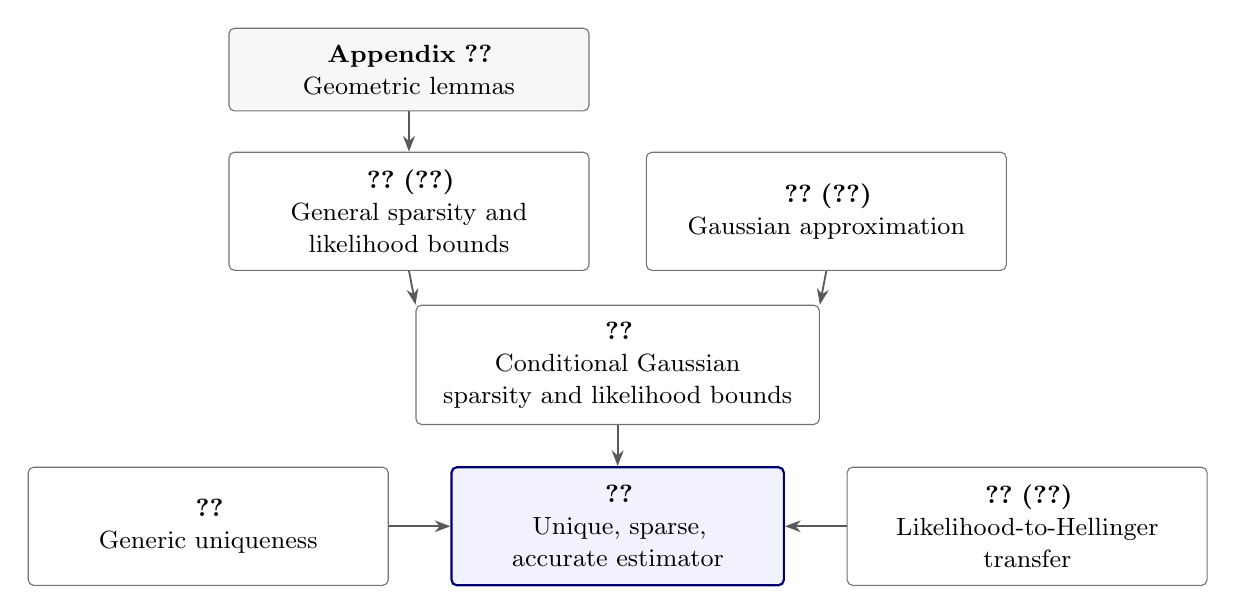
\begin{tikzpicture}[
  font=\small,
  result/.style={draw=black!55, rounded corners=2pt, align=center,
    text width=4.15cm, minimum height=1.05cm, inner sep=6pt},
  dependency/.style={-{Stealth[length=2mm]}, draw=black!65, line width=0.65pt}
]
\node[result, fill=black!3] (geometry) at (-2.65,0)
  {\textbf{Appendix~\ref{app:effective}}\\Geometric lemmas};
\node[result, minimum height=1.5cm] (effective) at (-2.65,-1.8)
  {\textbf{\Cref{thm:effective} (\Cref{sec:effective})}\\
   General sparsity and\\likelihood bounds};
\node[result, minimum height=1.5cm] (approximation) at (2.65,-1.8)
  {\textbf{\Cref{prop:gaussian-width} (\Cref{sec:gaussian})}\\
   Gaussian approximation};
\node[result, text width=4.7cm] (conditional) at (0,-3.75)
  {\textbf{\Cref{cor:conditional}}\\Conditional Gaussian\\
   sparsity and likelihood bounds};
\node[result, minimum height=1.5cm] (uniqueness) at (-5.2,-5.8)
  {\textbf{\Cref{prop:generic}}\\Generic uniqueness};
\node[result, text width=3.8cm, minimum height=1.5cm,
  draw=blue!45!black, fill=blue!5, line width=0.8pt] (main) at (0,-5.8)
  {\textbf{\Cref{thm:main}}\\Unique, sparse,\\accurate estimator};
\node[result, minimum height=1.5cm] (accuracy) at (5.2,-5.8)
  {\textbf{\Cref{thm:near-mle} (\Cref{sec:hellinger})}\\
   Likelihood-to-Hellinger\\transfer};
\draw[dependency] (geometry.south) -- (effective.north);
\draw[dependency] (effective.south) -- (conditional.north west);
\draw[dependency] (approximation.south) -- (conditional.north east);
\draw[dependency] (conditional.south) -- (main.north);
\draw[dependency] (uniqueness.east) -- (main.west);
\draw[dependency] (accuracy.west) -- (main.east);
\end{tikzpicture}
\caption{Structure of the proof of \Cref{thm:main}.  Arrows indicate inputs
to subsequent results.  The conditional Gaussian bounds and generic
uniqueness establish parts (i)--(iii); the likelihood-to-Hellinger transfer
completes part (iv).}
\label{fig:proof-roadmap}
\end{figure}
\fi

%======================================================================
\section{An effective-dimension principle for exact sparsity}
\label{sec:effective}
%======================================================================

Nothing in the support phenomenon is specific to Gaussian kernels.  This
section states an abstract result for any positive continuous kernel whose
fitted vectors have small linear approximation width.  Gaussian structure
enters only in \Cref{sec:gaussian}, through a sharp bound on that width.

\subsection{Positive kernel hulls and optimizer fibers}

Let $\Theta$ be a nonempty compact metric space and let
$A:\Theta\to(0,\infty)^n$ be continuous; in the Gaussian model, $\Theta=K$
and $A(\theta)=(\phi_d(x_i-\theta))_{i\le n}$.  Write
\[
 \Acal=A(\Theta),\qquad \Ccal=\conv(\Acal).
\]
The set $\Ccal$ consists exactly of the fitted vectors
$\int A(\theta)\,dG(\theta)$ with $G\in\Pcal(\Theta)$.  For
$w\in(0,\infty)^n$, define
\begin{equation}\label{eq:value}
 \Psi(w)=\max_{v\in\Ccal}w^\top\log v,
 \qquad
 \vhat(w)=\argmax_{v\in\Ccal}w^\top\log v,
 \qquad z(w)=\log\vhat(w).
\end{equation}
Because $v\mapsto w^\top\log v$ is strictly concave, the fitted vector
$\vhat(w)$ is unique.  The set of maximizing mixing measures is the
\emph{optimizer fiber}
\begin{equation}\label{eq:fiber}
 \Mcal_A(w)=\left\{G\in\Pcal(\Theta):
       \int A(\theta)\,dG(\theta)=\vhat(w)\right\}.
\end{equation}

Recall that a member of a convex set is \emph{extreme} if it is not a
nontrivial convex combination of two other members.  Our object of interest
is the largest support among extreme optimizers,
\begin{equation}\label{eq:sext}
 \sext(w)=
 \max\left\{\#\supp(G):G\text{ is an extreme point of }\Mcal_A(w)\right\}.
\end{equation}
This maximum is well defined and lies in $\{1,\ldots,n\}$, because an
optimizer is extreme exactly when it is finitely supported and its
evaluation vectors are linearly independent (\Cref{lem:extreme}).

\subsection{Effective dimension}

Sparsity will be controlled by how close the fitted vectors are to a
low-dimensional subspace, measured relative to the equal-weight fit.  Let
$v_0=\vhat(\one)$ and define the relative fitted-value set
\begin{equation}\label{eq:relative-set}
 \Ucal=\{v/v_0-\one:v\in\Ccal\}.
\end{equation}

\begin{definition}[Effective dimension and residual width]
A rank-$r$ orthogonal projection $P$ on $\RR^n$ has \emph{residual width}
$\eta$ if
\begin{equation}\label{eq:width}
 \sup_{u\in\Ucal}\norm{(I-P)u}_2\le\eta.
\end{equation}
We then call $r$ an effective linear dimension of $\Ucal$.  Both $r$ and
$\eta$ may depend on the fixed data and kernel dictionary, but not on the
random weights.
\end{definition}

We also need a notion of approximate optimality.  For $\tau\ge0$, a vector
$\vtil\in\Ccal$ is a \emph{$\tau$-optimal weighted fit} if
\begin{equation}\label{eq:tau-opt}
 w^\top\log\vtil\ge\Psi(w)-\tau,
\end{equation}
so that the tolerance is measured in units of total weighted log-likelihood.

\begin{theorem}[Effective-dimension exact sparsification]
\label{thm:effective}
There are universal constants $C,c>0$ such that the following holds.  Fix
$q\ge1$, put $Q=q+\log(2n)$, and suppose
\begin{equation}\label{eq:effective-conditions}
 \alpha\ge C(r+Q),
 \qquad
 \eta\sqrt{\alpha nQ}\le1.
\end{equation}
Let $W_i\stackrel{\mathrm{iid}}\sim\mathrm{Gamma}(\alpha,\alpha)$.  With
probability at least $1-3e^{-q}$,
\begin{equation}\label{eq:effective-support}
 \sext(W)\le C(r+q),
\end{equation}
\begin{equation}\label{eq:effective-exact-fit}
 0\le \one^\top\log v_0-\one^\top\log\vhat(W)
 \le\frac{C(r+q)}{\alpha},
 \qquad
 \norm{\log\{\vhat(W)/v_0\}}_2^2
 \le\frac{C(r+q)}{\alpha}.
\end{equation}
On the same event, simultaneously for every $0\le\tau<c$ and every
$\tau$-optimal fit $\vtil$,
\begin{equation}\label{eq:effective-approx-fit}
 0\le \one^\top\log v_0-\one^\top\log\vtil
 \le C\left\{\frac{r+q}{\alpha}+\tau\right\},
 \qquad
 \norm{\log(\vtil/v_0)}_2^2
 \le C\left\{\frac{r+q}{\alpha}+\tau\right\}.
\end{equation}
The support conclusion concerns exact extreme optimizers.  No support bound
is asserted for arbitrary approximate fitted measures.
\end{theorem}

The theorem shows how much randomization is needed.  The concentration
$\alpha$ need only exceed the effective dimension plus a logarithmic tail
cost.  Increasing $\alpha$ brings the objective closer to equal weighting but
demands a smaller residual width.  For Gaussian kernels, analyticity allows
both conditions to hold even when $\alpha$ is polynomially large.

\subsection{Why support is visible to the Hessian}

We close the section by explaining where the support bound
\eqref{eq:effective-support} comes from; the full argument is in
\Cref{app:effective}.  By \Cref{lem:regularity}, the value function $\Psi$
is convex and continuously differentiable with $\nabla\Psi=z$, and $z$ is
locally Lipschitz, so the Hessian $\nabla^2\Psi$ exists almost everywhere.
Now suppose an extreme optimizer has $k$ atoms.  Moving mass among these
atoms while keeping the total fixed produces a $(k-1)$-dimensional space of
perturbations of the fitted vector, each feasible in both directions.  A
second-order comparison turns these directions into curvature of $\Psi$.

\begin{lemma}[Support--sensitivity inequality]
\label{lem:hessian-summary}
The Hessian $\nabla^2\Psi(w)$ exists at almost every $w\in(0,\infty)^n$,
and the exceptional set depends only on the dictionary and not on a
selected optimizer.  At each point where it exists and for every extreme
optimizer $G\in\Mcal_A(w)$ with $k$ atoms, there is an orthogonal projection
$P_G$ of rank $k-1$ such that
$\diag(w)^{1/2}\nabla^2\Psi(w)\diag(w)^{1/2}\succeq P_G$.  In particular,
for almost every $w$ there is an orthogonal projection $P_*(w)$ of rank
$\sext(w)-1$ such that
\begin{equation}\label{eq:hessian-summary}
 \diag(w)^{1/2}\nabla^2\Psi(w)\diag(w)^{1/2}\succeq P_*(w).
\end{equation}
\end{lemma}

The proof is in \Cref{app:effective-local}.

This matrix inequality says more than a trace bound would: it produces a
determinant factor that is exponential in the support size.  To exploit it,
let
\[
 t(w)=z(w)-z(\one),
 \qquad Z(w)=(w-\one)^\top t(w),
\]
and consider the locally Lipschitz map $\mathcal F$ with coordinates
\begin{equation}\label{eq:change-map}
 \mathcal F_i(w)=w_i\{1+t_i(w)\}.
\end{equation}
On the event that the weighted fit is close to $v_0$, this map is injective,
and the determinant of its derivative contains the factor
$(17/9)^{\sext(w)-1}$.  Comparing the Gamma density at $\mathcal F(w)$ with
that at $w$ and applying the injective area formula \citep{evansgariepy2015}
gives
\begin{equation}\label{eq:moment-summary}
 \EE\left[\bm 1_{\{W\in E\}}
 \left(\frac{17}{9}\right)^{\sext(W)-1}
 e^{-\alpha\{Z(W)+\norm{t(W)}_2^2\}}\right]\le1
\end{equation}
for a suitable localization event $E$ (\Cref{lem:determinant-moment}).  The
width condition \eqref{eq:width} bounds the exponential cost in
\eqref{eq:moment-summary} by $O(r+q)$, and Markov's inequality then yields
\eqref{eq:effective-support}.  It is this change of variables that makes the
sparsity exact: it controls the number of atoms itself, rather than the size
of small mixture weights or an approximation error.

%======================================================================
\section{Gaussian effective dimension and generic uniqueness}
\label{sec:gaussian}
%======================================================================

We now specialize \Cref{thm:effective} to the Gaussian evaluation dictionary
\[
 A(\theta)=\bigl(\phi_d(x_1-\theta),\ldots,
                    \phi_d(x_n-\theta)\bigr),
 \qquad \theta\in K.
\]
Throughout this section the dataset $x=(x_1,\ldots,x_n)$ is fixed, and
$T=\max_i\norm{x_i}$ denotes its radius.

\subsection{Analytic low-rank approximation}

The identity
\[
 \phi_d(x_i-\theta)=\phi_d(x_i)
 \exp\{x_i^\top\theta-\norm{\theta}^2/2\}
\]
reduces the geometry of Gaussian fitted values to that of multivariate
exponential functions, and truncating their Taylor series yields the
required effective dimension.

\begin{proposition}[Gaussian relative-width bound]
\label{prop:gaussian-width}
Suppose that \Cref{ass:standing} holds and let $G_0\in\Pcal(K)$ be
arbitrary.  Put
$v_{0,i}=f_{G_0}(x_i)$.  For every integer $m\ge0$, there is an orthogonal
projection $P_m$ of rank at most
\begin{equation}\label{eq:rank-m}
 1+\binom{m+d}{d}
\end{equation}
whose range contains $\one$ and such that
\begin{equation}\label{eq:eta-m}
 \sup_{G\in\Pcal(K)}
 \norm{(I-P_m)\{f_G(x)/v_0-\one\}}_2
 \le \eta_m:=\sqrt n\,\eps_m,
\end{equation}
where
\begin{equation}\label{eq:eps-m}
 \eps_m=\exp(2ST+S^2/2)\frac{(ST)^{m+1}}{(m+1)!}.
\end{equation}
When $ST=0$, one may take $\eps_m=0$.
\end{proposition}

If $T\le C_0\sqrt{\log n}$ and $m\asymp\log n/\log\log n$, the rank bound
\eqref{eq:rank-m} is $O(r_n)$, while $\eps_m$ falls below any prescribed
inverse power of $n$ once the constant in $m$ is large enough.  The width
condition of \Cref{thm:effective} therefore holds over a wide range of
$\alpha$.  With the balanced concentration, we obtain the following bounds,
which are conditional on the data.

\begin{corollary}[Conditional structural and likelihood bounds]
\label{cor:conditional}
Suppose that \Cref{ass:standing} holds.  Fix $C_0<\infty$ and a dataset
with $T\le C_0\sqrt{\log n}$.  Let $r_n,\bar r_n$ be as in
\eqref{eq:scales}, set $\alpha_n=\bar r_n\log n$, and draw independent
$\mathrm{Gamma}(\alpha_n,\alpha_n)$ weights.  For every $b>0$, with
conditional probability at least $1-C_bn^{-b}$,
\[
 \sext(W)\le C_b\bar r_n,
 \qquad
 \max_i\abs{W_i-1}\le C_b\bar r_n^{-1/2},
\]
and every exact weighted maximizer satisfies the two bounds in
\Cref{thm:main}(iii).  These conclusions are deterministic in the data and
make no sampling or correct-specification assumption.
\end{corollary}

\subsection{From sparse extreme points to a unique measure}

A support bound on extreme points does not by itself make every optimizer
sparse, since a nontrivial convex combination of extreme optimizers can have
larger, or even infinite, support.  For Gaussian evaluations, generic data
rule this out once all extreme optimizers are sufficiently sparse.

\begin{proposition}[Generic evaluation independence]
\label{prop:generic}
For each $n,d$, there is a Borel set $\mathcal X_{n,d}\subset(\RR^d)^n$ whose
complement has Lebesgue measure zero such that the following holds
simultaneously for every $x\in\mathcal X_{n,d}$.  If
$k(d+1)\le n$ and $\theta_1,\ldots,\theta_k\in\RR^d$ are distinct, then the
$n\times k$ matrix
\begin{equation}\label{eq:evaluation-matrix}
 \bigl(\phi_d(x_i-\theta_j)\bigr)_{i\le n,j\le k}
\end{equation}
has linearly independent columns.  The locations may depend on the data.
Consequently, if every extreme point of a Gaussian optimizer fiber has at
most $m$ atoms and $2m(d+1)\le n$, then that fiber is a singleton and its
unique member has at most $m$ atoms.
\end{proposition}

What makes the proposition useful is that it holds simultaneously for all of
the uncountably many possible locations, including locations chosen after
seeing the data.  The proof views a linear dependence as a point of an
analytic incidence set with $k(d+1)-1$ free parameters.  Since this is fewer
than the $n$ equations imposed by the sample, the incidence set projects onto
a Lebesgue-null set of datasets.  Uniqueness then follows by comparing two
extreme optimizers and invoking the Krein--Milman theorem; the details are in
\Cref{app:generic}.

%======================================================================
\section{Hellinger accuracy from near-maximal likelihood}
\label{sec:hellinger}
%======================================================================

The previous two sections show that reweighting costs only $O(1/\log n)$ in
total ordinary log-likelihood.  This section converts that deterministic
near-optimality into a global density guarantee.  The argument is uniform by
design: a single data event controls every candidate whose log-likelihood is
within one unit of that of the truth.

\begin{theorem}[Uniform Hellinger control for near-MLEs]
\label{thm:near-mle}
Suppose that \Cref{ass:standing} holds and that the data follow
\eqref{eq:model}.  For every $b>0$, there are constants $C_b,n_0$ such that, uniformly over
$G^*\in\Pcal(K)$, with probability at least $1-C_bn^{-b}$ the following
holds simultaneously for all $G\in\Pcal(K)$:
\begin{equation}\label{eq:near-truth}
 L_n(G)\ge L_n(G^*)-1
 \quad\Longrightarrow\quad
 H^2(f_G,f_{G^*})
 \le C_b\frac{(\log n)^{d+1}}
 {n(\log\log n)^d}.
\end{equation}
\end{theorem}

The proof, given in \Cref{app:hellinger}, rests on a deterministic finite
net $\Ncal_n$ of the compact Gaussian mixture class that approximates
Hellinger distance globally and log densities on the sample-radius ball, and
whose size satisfies
\begin{equation}\label{eq:net-entropy-summary}
 \log\abs{\Ncal_n}
 \le C\frac{(\log n)^{d+1}}{(\log\log n)^d}.
\end{equation}
For each fixed net density $p$, the square-root likelihood ratio has
expectation
\[
 \EE_{G^*}\exp\left\{\frac12\sum_{i=1}^n
          \log\frac{p(X_i)}{f_{G^*}(X_i)}\right\}
 =\left(1-\frac12H^2(p,f_{G^*})\right)^n,
\]
so a union bound over the net rules out every Hellinger-distant candidate
whose log-likelihood ratio exceeds $-2$.

The approximate-fit bounds in \Cref{thm:effective} also have a practical
reading: the statistical guarantees survive inexact numerical optimization.

\begin{corollary}[Robustness to numerical optimization]
\label{cor:approx}
Under the setting and weighting of \Cref{thm:main}, suppose a fitted vector
$\vtil$ is attainable by a mixing law $\Gtil\in\Pcal(K)$ and has total
weighted log-likelihood gap $\tau_n\le c_0/\log n$, where $c_0$ is a fixed
sufficiently small constant.  Then, with probability at least $1-C_bn^{-b}$,
\[
 0\le L_n(\Ghat_0)-L_n(\Gtil)\le C_b/\log n,
 \qquad
 \sum_i\left\{\log\frac{f_{\Gtil}(X_i)}
 {f_{\Ghat_0}(X_i)}\right\}^2\le C_b/\log n,
\]
and $\Gtil$ obeys the Hellinger bound in \Cref{thm:main}(iv).  This result
does not assert exact sparsity of an arbitrary approximate optimizer.
\end{corollary}

%======================================================================
\section{Numerical evidence: sparsity and proximity to the ordinary NPMLE}
\label{sec:numerics}
%======================================================================

The theory is asymptotic and its main conclusion is structural, so the
simulations are not meant to exhibit a risk advantage over the ordinary
NPMLE.  They address three finite-sample questions: whether the reweighted
estimator keeps the density accuracy and support size of the ordinary
estimator, how quickly it approaches the ordinary fit as the perturbation
vanishes, and whether concentrating the weights is essential.  All
comparisons are paired on the same simulated dataset.\footnote{Numerical
means, standard errors, percentages, quantiles, and regression coefficients
are reported at the displayed precision.  Range endpoints described below as
rounded extrema are the rounded minimum and maximum cell summaries, not
literal enclosing bounds on the unrounded values.}

\subsection{Design and numerical validation}

We use three correctly specified Gaussian location-mixture models.  The first
is the one-dimensional three-point mixture
\[
 G^*=0.25\delta_{-2.5}+0.50\delta_0+0.25\delta_{2.5},
 \qquad K=[-4,4].
\]
The second uses the uniform mixing law $G^*=\operatorname{Unif}[-2.5,2.5]$ on
the same parameter space and checks that the conclusions do not depend on
finite true support.  The third is two-dimensional, with equal mass at the
four corners $(\pm1.75,\pm1.75)$ and $K=[-3.5,3.5]^2$.  The one-dimensional
designs use $n\in\{200,500,1000,2000\}$ with 100 replications each, and the
two-dimensional design uses $n\in\{250,500,1000\}$ with 40 replications.

We compare four estimators: the ordinary equal-weight NPMLE; the
\emph{balanced} estimator, with the concentration in \eqref{eq:scales}; the
\emph{tiny} estimator, with $\alpha_n=n^3$, which corresponds to
\Cref{cor:tiny} with $L=1/2$; and a \emph{BB-scale} control with $\alpha=1$.
The control is deliberately noisy and is not proposed as a point estimator;
it shows what happens when the weights are random but not increasingly
concentrated.  Each weight realization is normalized to
\[
 \widetilde W_i=\frac{W_i}{n^{-1}\sum_jW_j}=n\pi_i,
\]
which leaves the optimizer unchanged and removes an irrelevant common scale.

For each fit we record the numerical support size, the squared Hellinger risk
$H^2(f_{\widehat G},f_{G^*})$, the squared Hellinger distance to the ordinary
fit, the total ordinary-likelihood loss
$L_n(\widehat G_0)-L_n(\widehat G_W)$, and the squared fitted-log
discrepancy
\[
 \sum_{i=1}^n\left\{
 \log f_{\widehat G_W}(X_i)-\log f_{\widehat G_0}(X_i)
 \right\}^2.
\]
Hellinger integrals are computed on $[-10,10]$ using 6001 points in one
dimension and on $[-12,12]^2$ using a $211\times211$ grid in two dimensions.
We report the number of connected clusters of positive-mass atoms, joining
locations separated by less than $0.01$ in one dimension or $0.05$ in two
dimensions.  The optimizer also prunes negligible masses and merges nearby
locations during column generation and polishing; it then recomputes the
optimality diagnostic for the final fitted measure.  Thus reported support
is a numerical resolution convention, rather than a claim about exact atom
counts in floating-point arithmetic.

The estimator is computed by fully corrective column generation.  Given a
current mixing law $G$, the global optimality residual is
\begin{equation}\label{eq:numerical-kkt}
 \mathcal R_w(G)=
 \sup_{\theta\in K}\left[
 \frac{1}{\sum_iw_i}\sum_{i=1}^n
 w_i\frac{\phi_d(X_i-\theta)}{f_G(X_i)}-1
 \right],
\end{equation}
which is zero at an exact optimum.  In one dimension we search a dense mesh
and refine its local peaks; in two dimensions we use a rectangular mesh with
multistart continuous refinement.  After column generation, we jointly
polish atom locations and masses and reevaluate the diagnostic, including
all active support locations.  These searches approximate the supremum in
\eqref{eq:numerical-kkt}; they do not provide certified global upper bounds.
Across the \numReportedFits{} recorded fits (480 weighted path fits and
3680 Monte Carlo fits), the largest recorded residual was at most
$\numMaxResidual$, a conservatively upward-rounded bound; the
one-dimensional maximum rounded to $\numMaxResidualOneD$.  The additional
ordinary path baseline is recorded separately.  Ten dispersed random
initializations on representative one- and two-dimensional datasets gave
largest squared Hellinger discrepancies from their reference fits of
$\numMultistartDistanceOneD$ and $\numMultistartDistanceTwoD$, respectively.
An independent check reconstructs saved fits and compares denser oracle
searches and wider, finer integration grids.  These diagnostics support the
numerical comparison; they do not establish theoretical uniqueness or
certify a continuous global optimum.

All fitted locations, masses, data seeds, and weight seeds are retained.
For ordinary-likelihood loss we also retain the signed computed difference;
the figures and summary table display its nonnegative part.  There are
\numNegativeRawLossCount{} negative differences across the recorded fits,
with minimum $\numMinRawLoss$.  Such differences reflect optimization error,
and losses at this scale, especially in the tiny regime, should be read as
numerically unresolved rather than accurately measured positive losses.

\subsection{A regularization path}

We first fix one sample of size $n=500$ from the three-point mixture and vary
$\alpha$ from 1 to $n^3$, drawing 30 independent weight vectors at each
value.  \Cref{fig:path} reports medians and 10--90\% intervals.  The balanced
value for this experiment is $\alpha_n=\numPathBalancedAlpha$.

\begin{figure}[t]
\centering
\begin{minipage}[t]{0.48\textwidth}
  \centering\includegraphics[width=\linewidth]{numerics_v3/figures/path_weight_deviation.pdf}
  \par\vspace{-0.2em}\centerline{\small (a) Weight perturbation}
\end{minipage}\hfill
\begin{minipage}[t]{0.48\textwidth}
  \centering\includegraphics[width=\linewidth]{numerics_v3/figures/path_hellinger_to_ordinary.pdf}
  \par\vspace{-0.2em}\centerline{\small (b) Distance to the ordinary fit}
\end{minipage}

\par\medskip
\begin{minipage}[t]{0.48\textwidth}
  \centering\includegraphics[width=\linewidth]{numerics_v3/figures/path_likelihood_gap.pdf}
  \par\vspace{-0.2em}\centerline{\small (c) Ordinary-likelihood loss}
\end{minipage}\hfill
\begin{minipage}[t]{0.48\textwidth}
  \centering\includegraphics[width=\linewidth]{numerics_v3/figures/path_support.pdf}
  \par\vspace{-0.2em}\centerline{\small (d) Numerical support}
\end{minipage}
\caption{Regularization path on a fixed $n=500$ sample from the three-point
mixture.  Curves show medians across 30 independent Gamma-weight draws and
bands show the 10th and 90th percentiles.  The dashed and dotted vertical
lines mark the balanced concentration and $n^3$, respectively.}
\label{fig:path}
\end{figure}

The path exhibits two distinct rates.  A log--log regression of the medians
for $\alpha\ge10$ gives slope $\numSlopeWeight$ for $\max_i|\widetilde W_i-1|$,
matching the $\alpha^{-1/2}$ dispersion of Gamma weights.  The corresponding
slopes are $\numSlopeDistance$ for the squared Hellinger distance to the ordinary fit,
$\numSlopeLoss$ for the ordinary-likelihood loss, and $\numSlopeLogfit$ for the squared
fitted-log discrepancy.  The fitted vector thus moves at first order in the
weight perturbation, while the likelihood loss and the squared density
discrepancies are locally second order.

At the balanced concentration, the median squared Hellinger distance to the
ordinary fit is $\numPathBalancedDistance$ and the median total ordinary-likelihood
loss is $\numPathBalancedLoss$.  The ordinary fitted density has squared Hellinger risk
$\numPathOrdinaryRisk$ in this sample, against a median risk of $\numPathBalancedRisk$ for the
balanced estimator.  At $\alpha=n^3$, the distance and likelihood loss fall
to $\numPathTinyDistance$ and $\numPathTinyLoss$, and the risk agrees with the
ordinary risk to the displayed precision.  The median resolved support is
$\numPathBalancedMedianSupport$ atoms at the balanced concentration and
$\numPathTinyMedianSupport$ at the tiny concentration.  At the balanced value,
\numPathBalancedSupportSummary{}; at the tiny value,
\numPathTinySupportSummary{}.  By comparison, $\alpha=1$ yields a median distance of
$\numPathBBDistance$ and a median likelihood loss of $\numPathBBLoss$, with a
90th-percentile support of $\numPathBBUpperSupport$ atoms.

\begin{figure}[t]
\centering
\begin{minipage}[t]{0.49\textwidth}
  \centering\includegraphics[width=\linewidth]{numerics_v3/figures/representative_density.pdf}
  \par\vspace{-0.2em}\centerline{\small (a) Fitted densities}
\end{minipage}\hfill
\begin{minipage}[t]{0.49\textwidth}
  \centering\includegraphics[width=\linewidth]{numerics_v3/figures/representative_support.pdf}
  \par\vspace{-0.2em}\centerline{\small (b) Mixing measures}
\end{minipage}
\caption{Representative fits from the regularization-path experiment.  The
ordinary, balanced, and tiny fitted densities overlap closely,
although their atom locations and masses need not coincide exactly.  The
BB-scale fit exhibits a visible displacement.  For each weighted method,
we select the draw whose squared Hellinger distance to the ordinary fit is
closest to the within-concentration median.  Marker areas in panel (b) are
proportional to atom mass.}
\label{fig:representative}
\end{figure}

\Cref{fig:representative} shows why proximity is best judged through the
induced density, the fitted vector, and the likelihood.  At the balanced
concentration, the median one-dimensional Wasserstein distance between the
mixing laws is $\numPathBalancedWasserstein$, visibly larger than the discrepancy between the
convolved densities.  Gaussian deconvolution is an ill-posed inverse problem,
so a small perturbation of the density need not imply comparable
atom-by-atom stability in finite samples.  This is consistent with the
quantities that \Cref{thm:main} controls.

\subsection{Monte Carlo risk, support, and likelihood}

\Cref{tab:numerical-summary} reports the largest sample size in each design,
with Monte Carlo standard errors in parentheses, and \Cref{fig:risk} shows
the full sample-size trajectories.

\begin{table}[t]
\centering
\caption{Finite-sample comparison with the ordinary NPMLE.  ``Balanced'' uses
\eqref{eq:scales}, ``Tiny'' uses $\alpha_n=n^3$, and ``BB-scale'' uses
$\alpha=1$.  Entries are Monte Carlo means with standard errors in
parentheses.  Here $\Delta L_n=L_n(\widehat G_0)-L_n(\widehat G_W)$.}
\label{tab:numerical-summary}
\footnotesize
\setlength{\tabcolsep}{3.2pt}
\input{numerics_v3/results/numerical_summary.tex}
\end{table}

\begin{figure}[!tbp]
\centering
\begin{minipage}[t]{0.32\textwidth}
  \centering\includegraphics[width=\linewidth]{numerics_v3/figures/risk_three_point.pdf}
  \par\vspace{-0.2em}\centerline{\small (a) Three-point, $d=1$}
\end{minipage}\hfill
\begin{minipage}[t]{0.32\textwidth}
  \centering\includegraphics[width=\linewidth]{numerics_v3/figures/risk_uniform.pdf}
  \par\vspace{-0.2em}\centerline{\small (b) Uniform mixing, $d=1$}
\end{minipage}\hfill
\begin{minipage}[t]{0.32\textwidth}
  \centering\includegraphics[width=\linewidth]{numerics_v3/figures/risk_square_2d.pdf}
  \par\vspace{-0.2em}\centerline{\small (c) Four-point square, $d=2$}
\end{minipage}
\caption{Mean squared Hellinger risk as a function of sample size.  Shaded
bands show pointwise Monte Carlo means plus or minus 1.96 standard errors.}
\label{fig:risk}
\end{figure}

The balanced estimator tracks the ordinary NPMLE closely in every design.
Across all eleven design--sample-size cells, the ratio of mean Hellinger
risks has rounded minimum $\numBalancedRiskMin$ and rounded maximum $\numBalancedRiskMax$, with an
average across cells of $\numBalancedRiskAverage$.  The mean squared Hellinger distance
between the two fitted densities has rounded minimum $\numBalancedDistanceMin$ and
rounded maximum $\numBalancedDistanceMax$.  The resolved support counts of the two
estimators agree in $\numBalancedSupportAgreement\%$ of the \numPairedDatasets{} paired replications, and the mean
support difference in every cell lies between $\numBalancedSupportDifferenceMin$ and $\numBalancedSupportDifferenceMax$ atoms.
These comparisons show little support inflation over the designs studied.
Nor is its purpose to use fewer atoms than an ordinary NPMLE that already
happens to be sparse; what it adds is a generic, unique, sparse selection
backed by a quantitative guarantee.

The likelihood comparison matches the scale in \Cref{thm:main}(iii).  The
balanced mean total loss has rounded minimum $\numBalancedLossMin$ and rounded maximum
$\numBalancedLossMax$.  Multiplying the cell means by $\log n$ gives rounded minimum
$\numBalancedScaledLossMin$ and rounded maximum $\numBalancedScaledLossMax$; for the squared fitted-log discrepancy,
the corresponding rounded extrema are $\numBalancedScaledLogfitMin$ and $\numBalancedScaledLogfitMax$.  These constants
are stable across sample sizes and dimensions over the range studied.

The tiny regime is closer still.  Its ratio of mean Hellinger risk to
ordinary risk has rounded minimum $\numTinyRiskMin$ and rounded maximum $\numTinyRiskMax$,
and its mean squared Hellinger distance to the ordinary fit has rounded
minimum $\numTinyDistanceMin$ and rounded maximum $\numTinyDistanceMax$.  Its
resolved support count equals that of the ordinary estimator in
$\numTinySupportAgreement\%$ of the \numPairedDatasets{} paired replications at
the stated location resolution.  This is numerical evidence for the
message of \Cref{cor:tiny}: exact sparse selection can persist while the
objective and the fitted density become essentially indistinguishable from
their equal-weight counterparts.

The BB-scale control behaves quite differently.  Its ratio of mean Hellinger
risk to ordinary risk has rounded minimum $\numBBRiskMin$ and rounded maximum $\numBBRiskMax$,
and its mean total ordinary-likelihood loss has rounded minimum $\numBBLossMin$ and
rounded maximum $\numBBLossMax$.  It sometimes uses slightly fewer atoms, but at a
material statistical cost.  Randomization alone is thus not the relevant
regularizer; what matters is a continuous perturbation whose concentration
grows sufficiently quickly with $n$.

Taken together, the experiments support three conclusions.  First, the
balanced estimator retains the finite-sample density accuracy and support
complexity of the ordinary NPMLE.  Second, the inverse-polynomial regime can
make the two estimators operationally indistinguishable while retaining the
theoretical exact-sparsity guarantee.  Third, proximity concerns fitted
densities and likelihoods, rather than exact atom locations.

%======================================================================
\FloatBarrier
\section{Discussion}\label{sec:discussion}
%======================================================================

\paragraph{An estimator theorem.}
The central result is best read as a theorem about an estimator rather than
as a perturbation lemma.  Random reweighting produces a point estimator of
the mixing law with four simultaneous properties: exact polylogarithmic
support, generic uniqueness, asymptotically negligible loss of ordinary
likelihood, and global Hellinger convergence.  Each is needed.  Sparsity
alone could select a poor density, and Hellinger consistency alone would
leave the mixing representation nonunique and computationally unwieldy.  It
is the combination that makes the reweighted estimator statistically
meaningful.

\paragraph{Regularization without a penalty.}
No term depending on $\#\supp(G)$ appears in either the sample objective or
the population target.  The regularization is geometric: a small continuous
random tilt makes high-support optimizer fibers occupy little Gamma volume,
and the analytic effective dimension of Gaussian evaluations determines the
cardinality that remains.  Randomization thus acts as an exact support
regularizer without introducing an explicit regularization bias.

\paragraph{Auxiliary randomness.}
The guarantee requires only one draw of the weights; repeated bootstrap
optimization is neither part of the definition nor needed for the theory,
so the auxiliary seed can be fixed and recorded.  Different successful draws
may select different sparse mixing laws, but every such draw is close to the
ordinary fitted vector and lies in the same shrinking Hellinger neighborhood
of the truth.  The randomization is a reproducible regularization device,
not a tool for quantifying uncertainty.

\paragraph{Relation to self-regularization.}
The one-dimensional ordinary NPMLE is already known to have logarithmic
support under broad sampling conditions \citep{polyanskiywu2020}.  Our result
does not prove the analogous statement for the equal-weight multivariate
NPMLE\@.  It shows instead that an arbitrarily close objective has a unique
optimizer with a quantitative polylogarithmic support bound in every fixed
dimension.  The distinction is substantive, because upper bounds on support
do not pass to the equal-weight limit by lower semicontinuity.

\paragraph{Statistical rate.}
The Hellinger bound is near parametric up to logarithmic factors, but we do
not claim it is sharp.  For compact or sub-Gaussian Gaussian mixtures, known
lower bounds are of order $(\log n)^d/n$ under squared Hellinger loss
\citep{kimguntuboyina2022}, and local-entropy results sharpen the broader
minimax picture \citep{jiaetal2023}.  Improving the finite-net argument while
keeping a simultaneous guarantee for all near-MLE candidates is an important
direction.

\paragraph{Computation.}
The theory is structural; it is not a convergence theorem for an algorithm.
It implies that an exact extreme optimum has only polylogarithmically many
atoms and that a small objective error preserves fitted-value and Hellinger
accuracy.  The simulations show that fully corrective column generation,
followed by joint polishing of locations and masses, attains small numerically evaluated
Kiefer--Wolfowitz residuals while maintaining the predicted sparse
representation.  This supports exchange, vertex-direction, and adaptive
discretization methods, but it does not establish a general complexity bound
for them.  Using the Hessian response directions to obtain such a bound
remains an interesting algorithmic question.

\paragraph{Extensions.}
The effective-dimension theorem applies to general positive kernels.
Extending the full result to another model requires three ingredients: a
low-rank approximation of relative fitted values, generic evaluation
independence or another uniqueness mechanism, and a likelihood-to-risk
transfer for the induced density class.  Exponential families and
heteroscedastic Gaussian mixtures are natural candidates.  Derandomization, a
data-adaptive choice of $\alpha_n$, and the use of several sparse draws for
uncertainty quantification are further open problems.

\section*{Code and data availability}

The Python code for the solver and the numerical study, the raw simulation
output, and the scripts that produce every figure and table are provided as
ancillary files with the arXiv version of this paper.  All data-generating
and weight-draw seeds are deterministic and recorded in the code, so the
complete study can be rerun from the supplied commands.  A Lean~4
formalization of the theoretical results, written against mathlib, is
available at \leanrepo; its documentation describes the scope of
the verification.

% \section*{Acknowledgments}
% To be added.

\appendix
\crefalias{section}{appendix}
\crefalias{subsection}{appendix}

%======================================================================
\section{Proofs of the main results}
\label{app:main-proofs}
%======================================================================

This appendix assembles the proof of \Cref{thm:main} from the results of
\Cref{sec:effective,sec:gaussian,sec:hellinger} and proves
\Cref{cor:tiny,cor:weak,cor:approx}.  The supporting results are proved in
\Cref{app:effective,app:gaussian,app:hellinger,app:dirichlet}.

\subsection{Proof of Theorem~\ref{thm:main}}\label{app:proof-main}

\begin{proof}[Proof of \Cref{thm:main}]
Fix $b>0$.  All exceptional probabilities below are uniform over
$G^*\in\Pcal(K)$.

\emph{Step 1: the data event.}  Under \eqref{eq:model}, the joint
distribution of $(X_1,\ldots,X_n)$ has a density, so the generic event
$\{X\in\mathcal X_{n,d}\}$ of \Cref{prop:generic} has probability one.
Since $\norm{\Theta_i}\le S$, a Gaussian union bound gives
$\max_i\norm{X_i}\le C_b\sqrt{\log n}$ outside an event of probability
$O(n^{-b-2})$.  Let $\mathcal E_X$ denote the intersection of these two
events.

\emph{Step 2: parts \textup{(ii)} and \textup{(iii)}.}  On $\mathcal E_X$,
the dataset satisfies the hypothesis of \Cref{cor:conditional} with
$C_0=C_b$.  Hence, with conditional probability at least $1-C_bn^{-b}$ given
$X$, every extreme optimizer has at most $C_b\bar r_n$ atoms, the weights
satisfy $\max_i\abs{W_i-1}\le C_b\bar r_n^{-1/2}$, and every exact weighted
maximizer obeys both bounds in part (iii).  Integrating this conditional
bound over $\mathcal E_X$ proves parts (ii) and (iii) outside an event of
probability $C_bn^{-b}+O(n^{-b-2})$.

\emph{Step 3: uniqueness and part \textup{(i)}.}  Since $\bar r_n=o(n)$,
we have $2C_b\bar r_n(d+1)\le n$ for all sufficiently large $n$.  On the
event of Step 2 and on the generic event, the second part of
\Cref{prop:generic}, applied with $m=C_b\bar r_n$, shows that the weighted
optimizer fiber is a singleton whose unique member has at most $C_b\bar r_n$
atoms.  This proves part (i).

\emph{Step 4: part \textup{(iv)}.}  On the event of Step 2, part (iii) gives,
for all sufficiently large $n$,
\[
 L_n(\Ghat_W)\ge L_n(\Ghat_0)-1\ge L_n(G^*)-1,
\]
because $G^*$ is feasible for the ordinary likelihood.  On the event of
\Cref{thm:near-mle}, which has probability at least $1-C_bn^{-b}$, the
implication \eqref{eq:near-truth} then applies to $G=\Ghat_W$ and proves
part (iv).

\emph{Step 5: probability.}  The exceptional events of Steps 1, 2, and 4
have total probability at most $C_bn^{-b}$ after enlarging $C_b$, which
completes the proof.
\end{proof}

\subsection{Proofs of the corollaries}\label{app:proof-corollaries}

\begin{proof}[Proof of \Cref{cor:tiny}]
Take $\alpha_n=n^{2L+2}$ and work on the data event $\mathcal E_X$ of Step 1
in the proof of \Cref{thm:main}.

\emph{Sparsity and uniqueness.}  In \Cref{prop:gaussian-width}, choose
$m=\lceil C_L\log n/\log\log n\rceil$ with $C_L$ sufficiently large.  Then
$\rank(P_m)=O_L(r_n)$ and $\eps_m\le n^{-L-3}$.  With $q=(b+2)\log n$, both
conditions in \eqref{eq:effective-conditions} hold for all large $n$.  Hence
\Cref{thm:effective} shows that every extreme optimizer has
$O_{b,L}(\bar r_n)$ atoms, and \Cref{prop:generic} again gives uniqueness.

\emph{Size of the perturbation.}  \Cref{lem:gamma-concentration} and a union
bound give
\[
 \PP\{\max_i\abs{W_i-1}>t\}\le2n\exp(-\alpha_nt^2/4),
 \qquad 0<t\le1,
\]
and the choice $t=n^{-L}$ yields the bound $2ne^{-n^2/4}$.

\emph{Hellinger accuracy.}  \Cref{thm:effective} also gives a total
ordinary-likelihood gap of $C_{b,L}\bar r_n/n^{2L+2}=o(1)$.  The weighted
optimizer therefore satisfies the hypothesis of \eqref{eq:near-truth} for all
sufficiently large $n$.  Apply \Cref{thm:near-mle} and combine the
exceptional events.
\end{proof}

\begin{proof}[Proof of \Cref{cor:weak}]
By \Cref{thm:main}(iv), $H(f_{\Ghat_W},f_{G^*})\to0$ in probability, so
every subsequence has a further subsequence along which the convergence holds
almost surely.  By compactness of $\Pcal(K)$, we may pass to a further
subsequence with $\Ghat_W\Rightarrow G$ for some $G$.  Along it, the Gaussian
kernel is bounded and continuous, so $f_{\Ghat_W}(x)\to f_G(x)$ for every
$x$, while Hellinger convergence gives $L^1$ convergence to $f_{G^*}$.  Hence
$f_G=f_{G^*}$ almost everywhere.  Since
$\widehat f_G(t)=e^{-\norm{t}^2/2}\widehat G(t)$ and the Gaussian factor never
vanishes, $G=G^*$.  Every subsequential limit is therefore $G^*$.
\end{proof}

\begin{proof}[Proof of \Cref{cor:approx}]
Apply \eqref{eq:effective-approx-fit} with the Gaussian width construction
used in \Cref{cor:conditional}.  The ordinary-likelihood gap is eventually
below one, so \Cref{thm:near-mle} applies.
\end{proof}

%======================================================================
\section{Proof of the effective-dimension theorem}
\label{app:effective}
%======================================================================

This appendix proves \Cref{thm:effective} in four steps: basic regularity
of the fitted-vector problem (\Cref{app:effective-basic}), the Hessian
lower bound and localization of the weighted fit
(\Cref{app:effective-local}), the Gamma change of variables
(\Cref{app:effective-cov}), and the final probability estimates
(\Cref{app:effective-proof}).  Throughout, we use the setting of
\eqref{eq:value}--\eqref{eq:width}.

\subsection{Basic convex geometry}
\label{app:effective-basic}

\begin{lemma}[Regularity of the fitted-vector problem]
\label{lem:regularity}
In the setup of \eqref{eq:value}, $\Ccal$ is compact,
$\Psi$ is convex and continuously differentiable on $(0,\infty)^n$, and
\[
 \nabla\Psi(w)=z(w)=\log\vhat(w).
\]
The maps $w\mapsto\vhat(w)$ and $w\mapsto z(w)$ are locally Lipschitz.
All optimizing measures have fitted vector $\vhat(w)$.
\end{lemma}

\begin{proof}
Since $\Acal$ is compact in $\RR^n$, Carath\'eodory's theorem expresses
every point of $\conv(\Acal)$ as a convex combination of at most $n+1$
points of $\Acal$; hence $\Ccal$ is compact.  Positivity and compactness give
constants $0<\underline v\le\overline v<\infty$ such that
$\underline v\le v_i\le\overline v$ for all $v\in\Ccal$ and every $i$.  The
objective $v\mapsto\sum_iw_i\log v_i$ is continuous and strictly concave, so
it has a unique maximizing fitted vector.

Fix a compact box of weights in the positive
orthant and let $a_0>0$ be a common lower bound on its coordinates.  Put
$v=\vhat(w)$, $v'=\vhat(w')$, and $f_w(u)=\sum_iw_i\log u_i$.  Adding the
variational inequalities for the two maximizations gives
\[
 0\le\{\nabla f_w(v)-\nabla f_{w'}(v')\}^\top(v-v').
\]
Strong concavity of $f_w$ on $[\underline v,\overline v]^n$ and
$\nabla f_w(v')-\nabla f_{w'}(v')=(w-w')/v'$ imply
\[
 0\le-\frac{a_0}{\overline v^{\,2}}\norm{v-v'}_2^2
       +\frac1{\underline v}\norm{w-w'}_2\norm{v-v'}_2.
\]
Thus $\vhat$ is locally Lipschitz, and so is its coordinatewise logarithm.

As a maximum of linear functions of $w$, $\Psi$
is convex.  For small $h$, optimality at $w$ and at $w+h$ gives
\[
 h^\top z(w)\le\Psi(w+h)-\Psi(w)\le h^\top z(w+h).
\]
Continuity of $z$ yields differentiability of $\Psi$ with gradient $z$.
Finally, the weighted likelihood depends on a measure only through its
fitted vector in $\Ccal$, which proves the last assertion.
\end{proof}

\begin{lemma}[Extreme optimizer characterization]
\label{lem:extreme}
For every $w>0$, the fiber $\Mcal_A(w)$ in \eqref{eq:fiber} is nonempty,
compact, and convex.  A measure $G\in\Mcal_A(w)$ is extreme if and only if
\[
 G=\sum_{j=1}^kp_j\delta_{\theta_j},\qquad p_j>0,
\]
for finitely many distinct points whose evaluation vectors
$A(\theta_1),\ldots,A(\theta_k)$ are linearly independent.  Consequently,
every extreme optimizer has at most $n$ atoms.  The function
$\sext$ in \eqref{eq:sext} is Borel measurable.
\end{lemma}

\begin{proof}
\emph{Basic properties.}  Probability measures on compact $\Theta$ form a
compact convex set under weak convergence, and the continuous moment
constraints defining $\Mcal_A(w)$ are closed.  Nonemptiness follows from the
representation of $\vhat(w)\in\Ccal$ as a finite convex combination.

\emph{The contact identity.}  Let $\widehat v=\vhat(w)$ and define
\[
 \lambda_i=\frac{w_i}{\widehat v_i\sum_{\ell=1}^nw_\ell},
 \qquad q(\theta)=\lambda^\top A(\theta).
\]
The directional derivative of the weighted objective from $\widehat v$ toward
$A(\theta)$ is nonpositive, which gives $q(\theta)\le1$.  If $G$ is in the
fiber, then $\int q\,dG=\lambda^\top\widehat v=1$; hence $q=1$ on
$\supp(G)$.  Therefore, on an optimizing support, linear dependence and
affine dependence of the evaluation vectors are equivalent: applying
$\lambda^\top$ to a linear relation shows that its coefficients sum to zero.

\emph{Large support is not extreme.}  Suppose that $G$ has at least $n+1$
support points, including the case of infinite support.  Choose $n+1$
disjoint Borel neighborhoods $D_1,\ldots,D_{n+1}$ of positive $G$-mass.  The
vectors $a_j=\int_{D_j}A\,dG\in\RR^n$ are linearly dependent.  For
coefficients $c_j$, not all zero, with $\sum_jc_ja_j=0$, define the signed
measure $d\nu=\sum_jc_j\bm 1_{D_j}\,dG$.  Then $\int A\,d\nu=0$ and, because
$q=1$ $G$-almost surely, $\nu(\Theta)=\int q\,d\nu=0$.  For sufficiently
small $t>0$, both $G+t\nu$ and $G-t\nu$ are distinct probability measures in
the same fiber, so $G$ is not extreme.

\emph{Finite support.}  If $G$ has finite support but the evaluation vectors
are dependent, take a nonzero relation $\sum_jc_jA(\theta_j)=0$.  The contact
identity implies $\sum_jc_j=0$, and small perturbations $p_j\pm tc_j$ again
decompose $G$ inside the fiber.  Conversely, if the evaluation vectors are
linearly independent and $G=tG_1+(1-t)G_2$ with $G_1,G_2$ in the fiber, then
nonnegativity forces both measures to be supported on $\supp(G)$.  Their
masses solve the same full-rank linear system, so $G_1=G_2=G$.  This proves
the characterization and the $n$-atom bound.

\emph{Measurability.}  Let $\mathcal W_k$ be the set of weights admitting an
extreme optimizer with exactly $k$ atoms.  For integers $j\ge2$, consider the
compact set of $(w,\theta_1,\ldots,\theta_k,p)$ in
$[1/j,j]^n\times\Theta^k\times\Delta_k$ satisfying
\[
 p_\ell\ge1/j,\qquad
 \sum_{\ell=1}^kp_\ell A(\theta_\ell)=\vhat(w),
 \qquad \det(V^\top V)\ge1/j,
\]
where $V$ has columns $A(\theta_\ell)$.  Its projection onto $w$ is compact.
Taking the countable union over $j$ gives $\mathcal W_k$.  Hence
$\{w:\sext(w)\ge k\}=\bigcup_{\ell=k}^n\mathcal W_\ell$ is Borel for each
$k$.
\end{proof}

\subsection{Support directions and radial localization}
\label{app:effective-local}

We first prove the support--sensitivity inequality stated in
\Cref{sec:effective}.

\begin{proof}[Proof of \Cref{lem:hessian-summary}]
By \Cref{lem:regularity}, $z=\nabla\Psi$ is locally Lipschitz, so
Rademacher's theorem gives differentiability almost everywhere.  At those
points its derivative is the symmetric positive semidefinite Hessian of the
convex function $\Psi$.

Fix such a point and an extreme optimizer
$G=\sum_{j=1}^kp_j\delta_{\theta_j}$.  Write $A_j=A(\theta_j)$ and
$\widehat v=\vhat(w)$.  Varying the masses while preserving their sum
generates the relative fitted-vector subspace
\[
 \mathcal S=\left\{
 \left(\frac{\sum_jc_jA_{ij}}{\widehat v_i}\right)_{i=1}^n:
 \sum_jc_j=0\right\}.
\]
By \Cref{lem:extreme}, the evaluation vectors are linearly, hence affinely,
independent; therefore $\dim(\mathcal S)=k-1$.  Every sufficiently small
element of $\mathcal S$ is feasible in both signs, by changing only the
positive masses.  First-order optimality gives $w^\top u=0$ for
$u\in\mathcal S$.

Let $P_G$ be the orthogonal projection onto $\diag(w)^{1/2}\mathcal S$.  For
small $h$, choose the feasible relative variation
$u=\diag(w)^{-1/2}P_G\diag(w)^{-1/2}h$, that is, the candidate fitted vector
$\widehat v(\one+u)$.  Expanding its objective at weight $w+h$ gives
\[
 \Psi(w+h)\ge\Psi(w)+h^\top z(w)
 +h^\top u-\frac12u^\top\diag(w)u+o(\norm{h}_2^2).
\]
Because $w^\top u=0$, the two quadratic terms combine to
\[
 \frac12h^\top\diag(w)^{-1/2}P_G\diag(w)^{-1/2}h.
\]
Comparison with the second-order expansion of $\Psi$ at $w$ yields
$\nabla^2\Psi(w)\succeq\diag(w)^{-1/2}P_G\diag(w)^{-1/2}$, and conjugation by
$\diag(w)^{1/2}$ proves the claim.  The exceptional set is the
nondifferentiability set of $z$, which does not depend on the optimizer.
Choosing an extreme optimizer that attains $\sext(w)$ gives the final
statement.
\end{proof}

For the localization argument, retain \eqref{eq:relative-set}--\eqref{eq:width}
and write
\[
 \xi=w-\one,\qquad \omega_P=\norm{P\xi}_2,\qquad \omega=\norm{\xi}_2,
 \qquad \rho=\frac1{16}.
\]
Here $\omega_P$ is the part of the weight perturbation that is visible in the
effective subspace and $\omega$ is its total size.  For $u\in\Ucal$, let
$t(u)=\log(\one+u)$ and $F_w(u)=w^\top t(u)$, so that
$F_w(u)=w^\top\log v-w^\top\log v_0$ when $u=v/v_0-\one$.  For the exact
fit, write $\widehat u(w)=\vhat(w)/v_0-\one$, $t(w)=t(\widehat u(w))$, and
$Z(w)=\xi^\top t(w)$; these agree with the definitions in
\Cref{sec:effective}.

\begin{lemma}[Radial localization]
\label{lem:radial}
Let
\begin{equation}\label{eq:localization-event}
 E=\left\{w>0:
\norm{w-\one}_\infty\le\frac1{16},\quad
 \omega_P\le\frac{\rho}{24},\quad \eta\,\omega\le\frac{\rho^2}{24}\right\}.
\end{equation}
For $w\in E$, every $0\le\tau<\rho^2/12$ and every $\tau$-optimal fit with
relative vector $u=\vtil/v_0-\one$ satisfy $\norm{u}_2<\rho$ and
\begin{align}
 \norm{u}_2^2&\le36\omega_P^2+12\eta\omega+12\tau,\label{eq:radial-u}\\
 0\le-\one^\top\log(\one+u)
 &\le37\omega_P^2+13\eta\omega+13\tau,\label{eq:radial-loss}\\
 \norm{\log(\one+u)}_2^2
 &\le72\omega_P^2+24\eta\omega+24\tau.\label{eq:radial-log}
\end{align}
For the exact fit, $0\le Z(w)\le37\omega_P^2+13\eta\omega$.  The set $E$ is
compact and $\norm{t(w)}_\infty<1/8$ on $E$.
\end{lemma}

\begin{proof}
\emph{A quadratic upper bound.}  Equal-weight optimality at $v_0$ implies
$\one^\top u\le0$ for every $u\in\Ucal$.  If $\norm{u}_2\le1/4$, then
$\log(1+s)\le s-s^2/3$ coordinatewise.  On $E$, every $w_i\ge15/16$, so
\[
 F_w(u)\le \one^\top u+\xi^\top u-\frac{15}{48}\norm{u}_2^2
 \le \xi^\top u-\frac16\norm{u}_2^2
 \le \omega_P\norm{u}_2+\eta\,\omega-\frac16\norm{u}_2^2,
\]
where the last step splits
$\xi^\top u=(P\xi)^\top u+\xi^\top(I-P)u$ and uses \eqref{eq:width}.

\emph{Localization.}  On the sphere $\norm{u}_2=\rho$, the conditions
defining $E$ give $F_w(u)\le\rho^2/24+\rho^2/24-\rho^2/6=-\rho^2/12$ for
every feasible $u$.  A $\tau$-optimal fit has $F_w(u)\ge-\tau$ because
$u=0$ is feasible.  If $\norm{u}_2\ge\rho$, convexity of $\Ucal$ and
concavity of $F_w$ allow radial contraction of $u$ to the sphere without
decreasing $F_w$ below $-\tau$, contradicting $\tau<\rho^2/12$.  Hence
$\norm{u}_2<\rho$.

\emph{Quantitative bounds.}  Let $y=\norm{u}_2$.  The quadratic upper bound
and $F_w(u)\ge-\tau$ give $y^2\le6(\omega_Py+\eta\omega+\tau)$.  The bound
$6\omega_Py\le y^2/2+18\omega_P^2$ proves \eqref{eq:radial-u}.  For
$\abs{u_i}<\rho$,
\[
 \abs{\log(1+u_i)}\le\frac{\abs{u_i}}{1-\rho},
 \qquad
 \abs{\log(1+u_i)-u_i}\le\frac{u_i^2}{2(1-\rho)}\le u_i^2.
\]
The first inequality and \eqref{eq:radial-u} prove \eqref{eq:radial-log}.
Moreover,
\[
 \xi^\top\log(\one+u)
 \le \omega_Py+\eta\,\omega+\frac1{16}y^2
 \le37\omega_P^2+13\eta\omega+12\tau,
\]
where the constants are enlarged after applying Young's inequality and
\eqref{eq:radial-u}.  Since
$F_w(u)=\one^\top\log(\one+u)+\xi^\top\log(\one+u)\ge-\tau$, and
equal-weight optimality gives $-\one^\top\log(\one+u)\ge0$, we obtain
\eqref{eq:radial-loss}.  For the exact fit, $F_w(\widehat u)\ge0$ gives
$Z(w)\ge-\one^\top t(w)\ge0$ together with the stated upper bound.

\emph{Compactness.}  The set $E$ is closed inside $[15/16,17/16]^n$, hence
compact.  For the exact fit,
$\norm{t(w)}_\infty\le\norm{\widehat u(w)}_2/(1-\rho)<1/15<1/8$.
\end{proof}

\subsection{The Gamma change of variables}
\label{app:effective-cov}

\begin{lemma}[Determinant moment]
\label{lem:determinant-moment}
Let $E$ be the event in \eqref{eq:localization-event}.  For independent
$W_i\sim\mathrm{Gamma}(\alpha,\alpha)$,
\begin{equation}\label{eq:determinant-moment}
 \EE\left[\bm 1_{\{W\in E\}}
 \left(\frac{17}{9}\right)^{\sext(W)-1}
 \exp\{-\alpha[Z(W)+\norm{t(W)}_2^2]\}\right]\le1.
\end{equation}
\end{lemma}

\begin{proof}
\emph{Injectivity.}  On the open set
$U=\{w>0:1+t_i(w)>0\ \text{for all }i\}$, define the map $\mathcal F$ in
\eqref{eq:change-map}.  It is locally Lipschitz by \Cref{lem:regularity}.
Suppose $\mathcal F(w)=\mathcal F(w')=y$.  Then $w_i=y_i/\{1+t_i(w)\}$,
$w_i'=y_i/\{1+t_i(w')\}$, and, since $z(w)-z(w')=t(w)-t(w')$,
\[
 (w-w')^\top\{z(w)-z(w')\}
 =-\sum_i\frac{y_i\{t_i(w)-t_i(w')\}^2}
 {[1+t_i(w)][1+t_i(w')]}\le0.
\]
The gradient of the convex function $\Psi$ is monotone, so the left side is
nonnegative.  Hence $t(w)=t(w')$, and then $w=w'$.  Thus $\mathcal F$ is
injective on $U$.

\emph{Jacobian lower bound.}  At a point where the Hessian exists, let
\[
 D_t=\diag(\one+t(w)),\qquad
 R_w=\diag(w)^{1/2}\nabla^2\Psi(w)\diag(w)^{1/2}.
\]
Since $D_t$ is diagonal, the derivative
$D\mathcal F=D_t+\diag(w)\nabla^2\Psi(w)
=\diag(w)^{1/2}(D_t+R_w)\diag(w)^{-1/2}$ is similar to $D_t+R_w$.  By
\Cref{lem:hessian-summary}, $R_w\succeq P_*$ for an orthogonal projection
$P_*=VV^\top$ of rank $\sext(w)-1$, where $V$ has orthonormal columns.  On
$E$, \Cref{lem:radial} gives $7I/8\preceq D_t\preceq9I/8$, so
$V^\top D_t^{-1}V\succeq8I/9$.  Monotonicity of the determinant on positive
definite matrices, together with the fact that
$D_t^{-1/2}VV^\top D_t^{-1/2}$ and $V^\top D_t^{-1}V$ have the same nonzero
eigenvalues, yields
\[
 \det(D_t+R_w)\ge\det(D_t+VV^\top)
 =\det(D_t)\det(I+V^\top D_t^{-1}V),
\]
and therefore
\begin{equation}\label{eq:jacobian-lower}
 \det D\mathcal F(w)
 \ge\prod_i\{1+t_i(w)\}
 \left(\frac{17}{9}\right)^{\sext(w)-1}>0.
\end{equation}

\emph{Density ratio.}  Let $p_\alpha$ be the product Gamma density.  Since
$\mathcal F_i(w)=w_i\{1+t_i(w)\}$,
\[
 \frac{p_\alpha(\mathcal F(w))}{p_\alpha(w)}
 =\prod_i\{1+t_i(w)\}^{\alpha-1}
   \exp\left\{-\alpha\sum_iw_it_i(w)\right\}.
\]
Multiply by \eqref{eq:jacobian-lower}, write
$\sum_iw_it_i=\one^\top t+Z$, and use $\log(1+t)\ge t-t^2$ for
$\abs{t}\le1/8$.  This gives, almost everywhere on $E$,
\[
 \frac{p_\alpha(\mathcal F(w))\det D\mathcal F(w)}{p_\alpha(w)}
 \ge\left(\frac{17}{9}\right)^{\sext(w)-1}
 e^{-\alpha\{Z(w)+\norm{t(w)}_2^2\}}.
\]

\emph{Area formula.}  The set $E$ is compact and lies inside $U$.  The
injective area formula for Lipschitz maps
\citep[Chapter 3]{evansgariepy2015} therefore gives
\[
 \int_Ep_\alpha(\mathcal F(w))\abs{\det D\mathcal F(w)}\,dw
 =\int_{\mathcal F(E)}p_\alpha(y)\,dy\le1.
\]
The determinant is positive almost everywhere on $E$.  Integrating the
previous lower bound against $p_\alpha$ over $E$ proves
\eqref{eq:determinant-moment}.
\end{proof}

\subsection{Proof of the effective-dimension theorem}
\label{app:effective-proof}

\begin{proof}[Proof of \Cref{thm:effective}]
\emph{Concentration of the visible perturbation.}  Let $\xi=W-\one$ and put
$N_q=r\log5+q$.  The Gamma moment-generating function implies that, for
every deterministic unit vector $v$ and $\abs{\lambda}\le\sqrt\alpha/2$,
\[
 \log\EE e^{\lambda\sqrt\alpha\,v^\top\xi}
 =\alpha\sum_i\left[-\log\left(1-\frac{\lambda v_i}{\sqrt\alpha}\right)
 -\frac{\lambda v_i}{\sqrt\alpha}\right]\le\lambda^2.
\]
Consequently, $\PP\{\sqrt\alpha\,v^\top\xi>u\}\le e^{-u^2/4}$ for
$0\le u\le\sqrt\alpha$.  A $1/2$-net of the unit sphere in the
$r$-dimensional range of $P$ has at most $5^r$ points and satisfies
$\norm{y}_2\le2\max_v v^\top y$ for $y$ in that range.  Hence
\begin{equation}\label{eq:proj-concentration}
 \PP\{\alpha\norm{P\xi}_2^2>16N_q\}\le e^{-q}
\end{equation}
provided $\alpha\ge4N_q$.

\emph{Coordinatewise concentration.}  The scalar Gamma Chernoff bound gives
\[
 \PP\{\norm{\xi}_\infty>2\sqrt{Q/\alpha}\}
 \le2n e^{-Q}=e^{-q}
\]
when $\alpha\ge4Q$.  Let $E_q$ be the intersection of these two events.
Then $\PP(E_q^c)\le2e^{-q}$ and, on $E_q$,
\[
 \omega_P\le4\sqrt{N_q/\alpha},\qquad
 \omega\le2\sqrt{nQ/\alpha},\qquad
 \eta\,\omega\le2/\alpha,
\]
where the last inequality uses \eqref{eq:effective-conditions}.  Taking the
universal constant in \eqref{eq:effective-conditions} sufficiently large
ensures $E_q\subset E$, with $E$ as in \eqref{eq:localization-event}.

\emph{Likelihood bounds.}  Apply \Cref{lem:radial}.  Since
$N_q\le C(r+q)$, its exact-fit bounds yield
\[
 0\le\one^\top\log v_0-\one^\top\log\vhat(W)
 \le C\frac{r+q}{\alpha},
 \qquad
 \norm{\log\{\vhat(W)/v_0\}}_2^2
 \le C\frac{r+q}{\alpha}.
\]
The same lemma gives \eqref{eq:effective-approx-fit} simultaneously for all
$\tau<c$, after taking $c=\rho^2/12$ and enlarging $C$.

\emph{Support bound.}  Adding the exact-fit bounds of \Cref{lem:radial} for
$Z(W)$ and for $\norm{t(W)}_2^2$ gives, on $E_q$,
\[
 \alpha\{Z(W)+\norm{t(W)}_2^2\}
 \le109\alpha\omega_P^2+37\alpha\eta\omega
 \le1744N_q+74=:\Lambda_q.
\]
Set $\kappa=\log(17/9)$.  By \Cref{lem:determinant-moment} and Markov's
inequality,
\[
 \PP\{E_q,\ (\sext(W)-1)\kappa>\Lambda_q+q\}\le e^{-q}.
\]
Adding $\PP(E_q^c)$ shows that, outside probability $3e^{-q}$,
\[
 \sext(W)
 \le1+\frac{1744N_q+74+q}{\kappa}
 \le C(r+q).
\]
All conclusions hold on the same event.
\end{proof}

%======================================================================
\section{Gaussian approximation and uniqueness}
\label{app:gaussian}
%======================================================================

\subsection{Proof of the Gaussian relative-width bound}

\begin{proof}[Proof of \Cref{prop:gaussian-width}]
Set $\gamma_i=\phi_d(x_i)/v_{0,i}$.  The
Gaussian identity gives
\begin{equation}\label{eq:gaussian-ratio}
 \frac{\phi_d(x_i-\theta)}{v_{0,i}}
 =\gamma_i e^{-\norm{\theta}^2/2}e^{x_i^\top\theta}.
\end{equation}
Because
\[
 \frac{v_{0,i}}{\phi_d(x_i)}
 =\int e^{x_i^\top\vartheta-\norm{\vartheta}^2/2}\,dG_0(\vartheta)
 \ge e^{-ST-S^2/2},
\]
we have $\gamma_i\le e^{ST+S^2/2}$.  For $\abs{s}\le ST$, Taylor's theorem
yields
\[
 \left|e^s-\sum_{j=0}^m\frac{s^j}{j!}\right|
 \le e^{ST}\frac{(ST)^{m+1}}{(m+1)!}.
\]
Applying this with $s=x_i^\top\theta$ and multiplying by the remaining
factors in \eqref{eq:gaussian-ratio} shows that
\[
 \gamma_i e^{-\norm{\theta}^2/2}
 \sum_{j=0}^m\frac{(x_i^\top\theta)^j}{j!}
\]
approximates $\phi_d(x_i-\theta)/v_{0,i}$ with coordinatewise error at most
$\eps_m$ in \eqref{eq:eps-m}, uniformly over $i$ and $\theta\in K$.

The multinomial expansion of
$(x_i^\top\theta)^j$ uses only monomials $x_i^\beta$ with multi-index
$\abs{\beta}\le m$.  Hence every truncated vector lies in the span of
\[
 \left\{(\gamma_ix_i^\beta)_{i=1}^n:\abs{\beta}\le m\right\},
\]
whose dimension is at most $\binom{m+d}{d}$.  Adjoin $\one$ to this span and
let $P_m$ be the orthogonal projection onto the resulting subspace; its rank
obeys \eqref{eq:rank-m}.  Integrating the coordinatewise approximation under
any $G\in\Pcal(K)$ preserves its error, so $f_G(x)/v_0$ lies within
coordinatewise distance $\eps_m$, hence Euclidean distance
$\sqrt n\,\eps_m$, of the range of $P_m$.  Since
$\one$ also lies in that range and orthogonal projection minimizes Euclidean
distance to the subspace, \eqref{eq:eta-m} follows.  If $ST=0$, the
exponential term is constant in the relevant inner product and the expansion
is exact.
\end{proof}

\subsection{Proof of the conditional Gaussian corollary}

\begin{proof}[Proof of \Cref{cor:conditional}]
Choose any ordinary NPMLE $\Ghat_0$
and let $v_0=(f_{\Ghat_0}(x_i))_{i=1}^n$; by \Cref{lem:regularity}, this
vector does not depend on the chosen maximizing representation.  Apply
\Cref{prop:gaussian-width} with
\[
 m=\left\lceil C_m\frac{\log n}{\log\log n}\right\rceil,
\]
where $C_m>8$ is a sufficiently large constant depending only on the fixed
parameters.  The factorial inequality $(m+1)!\ge\{(m+1)/e\}^{m+1}$ and
$T\le C_0\sqrt{\log n}$ give
\begin{align*}
 \log\eps_m
 &\le 2ST+S^2/2+(m+1)\log\frac{eST}{m+1}\\
 &\le-3\log n
\end{align*}
for all sufficiently large $n$.  Indeed,
$\log(ST)\le\tfrac12\log\log n+O(1)$, whereas
$\log(m+1)=\log\log n-\log\log\log n+O(1)$.  If $ST=0$, the error is zero.
Thus
\[
 r:=\rank(P_m)=O(r_n),\qquad
 \eta:=\eta_m\le n^{-5/2}.
\]

Take
$q=(b+2)\log n$ and $Q=q+\log(2n)$.  Then $r+Q=O_b(\bar r_n)$ and
\[
 \frac{\alpha_n}{r+Q}\asymp_b\log n\to\infty.
\]
Moreover,
\[
 \eta\sqrt{\alpha_n nQ}
 \le n^{-5/2}\sqrt{\bar r_n\log n\cdot nQ}=o(1).
\]
The hypotheses of \Cref{thm:effective} therefore hold.  Its failure
probability is at most $3n^{-b-2}$, and it yields $\sext(W)\le C_b\bar r_n$
together with the likelihood and fitted-vector conclusions.

By \Cref{lem:gamma-concentration},
\begin{equation}\label{eq:gamma-coordinate}
 \PP\{\abs{W_i-1}>t\}\le2e^{-\alpha_nt^2/4},
 \qquad 0<t\le1.
\end{equation}
Choose $t=C_b'/\sqrt{\bar r_n}$ with $(C_b')^2/4\ge b+3$.  Since
$\alpha_nt^2=(C_b')^2\log n$, a union bound gives
\[
 \PP\{\max_i\abs{W_i-1}>t\}
 \le2n^{1-(C_b')^2/4}\le2n^{-b-2}.
\]
Intersect the events and enlarge constants.
\end{proof}

\subsection{Proof of generic evaluation independence}
\label{app:generic}

\begin{proof}[Proof of \Cref{prop:generic}]
\emph{Parametrizing dependences.}  Fix an integer $k$ satisfying
$k(d+1)\le n$.  A nonzero linear dependence among $k$ Gaussian evaluation
columns has a coefficient vector with at least one nonzero coordinate.
Normalize that coordinate to one; there are only $k$ possible choices.  In
one such chart, collect the $kd$ location coordinates and the remaining
$k-1$ coefficients in a parameter $\zeta\in\mathcal O\subset\RR^p$, where
\[
 p=kd+k-1=k(d+1)-1<n.
\]
The domain $\mathcal O$ is open after imposing distinctness of the
locations.  For the normalized coefficient vector $(c_1,\ldots,c_k)$, define
\[
 g_\zeta(y)=\sum_{j=1}^kc_j\phi_d(y-\theta_j),\qquad y\in\RR^d.
\]
This function is jointly real analytic in $(\zeta,y)$.

\emph{Nontriviality.}  For every admissible $\zeta$, $g_\zeta$ is not
identically zero.  Choose $v\in\RR^d$ such that the scalars $v^\top\theta_j$
are distinct; the excluded $v$ lie in finitely many proper hyperplanes.  If
$g_\zeta(sv)=0$ for every $s\in\RR$, then after division by the positive
common Gaussian factor,
\[
 \sum_{j=1}^kc_j e^{-\norm{\theta_j}^2/2}e^{s v^\top\theta_j}=0
 \qquad\text{for all }s.
\]
Differentiating at $s=0$ for orders $0,\ldots,k-1$ gives a Vandermonde
system with distinct nodes $v^\top\theta_j$, forcing every coefficient to
vanish.  This contradicts the normalization.

\emph{Dimension count.}  Consider the incidence set
\[
 I=\{(\zeta,x_1,\ldots,x_n)\in \mathcal O\times(\RR^d)^n:
        g_\zeta(x_i)=0\text{ for all }i\}.
\]
At an incidence point, analyticity and nontriviality imply that for each $i$
there is a multi-index $\mu_i$ of minimal total order with
$\partial_y^{\mu_i}g_\zeta(x_i)\ne0$.  Its order is at least one because
$g_\zeta(x_i)=0$.  Choose a coordinate $\ell_i$ with $\mu_{i,\ell_i}>0$ and
put $\mu_i'=\mu_i-e_{\ell_i}$.  By minimality,
\[
 h_i(\zeta,x_i):=\partial_y^{\mu_i'}g_\zeta(x_i)=0,
 \qquad
 \partial_{x_{i,\ell_i}}h_i(\zeta,x_i)\ne0.
\]
For each fixed choice of the countably many derivative indices, restrict to
the open region on which the displayed derivatives are nonzero.  The
Jacobian of $(h_1,\ldots,h_n)$ with respect to the selected data coordinates
$(x_{1,\ell_1},\ldots,x_{n,\ell_n})$ is diagonal and nonsingular.  The
implicit-function theorem therefore places the corresponding part of $I$ in
a smooth submanifold of codimension $n$ in $\mathcal O\times\RR^{nd}$, of
dimension
\[
 nd+p-n<nd.
\]
Each such submanifold has a countable atlas.  On compact subsets of a chart,
projection to the $nd$ data coordinates is Lipschitz, and the image of a
bounded set of dimension $D<nd$ under a Lipschitz map has zero
$nd$-dimensional Lebesgue measure.  Thus the projection of $I$ onto the data
coordinates is contained in a countable union of null sets.

Taking the finite union over coefficient normalizations
and over admissible $k$ produces a Borel null set $N_{n,d}$.  Let
$\mathcal X_{n,d}=(\RR^d)^n\setminus N_{n,d}$.  This proves the simultaneous
column-independence assertion.

For the final statement, suppose every extreme optimizer has at most $m$
atoms and $2m(d+1)\le n$.  If two distinct extreme optimizers existed, their
difference would be a nonzero signed measure on at most $2m$ distinct
locations with zero Gaussian evaluation vector.  After deleting zero
coefficients, this would contradict the independence just established.
Hence the compact convex optimizer fiber has at most one extreme point.  By
the Krein--Milman theorem it is the closed convex hull of its nonempty set of
extreme points, so it is a singleton.  Its unique member is extreme and has
at most $m$ atoms.
\end{proof}

%======================================================================
\section{Likelihood nets and Hellinger transfer}
\label{app:hellinger}
%======================================================================

\subsection{A finite Gaussian-mixture likelihood net}

\begin{lemma}[Simultaneous Hellinger and log-likelihood net]
\label{lem:finite-net}
Suppose that \Cref{ass:standing} holds and fix $b>0$.  For all
sufficiently large $n$, there are a deterministic finite set
$\Ncal_n\subset\{f_G:G\in\Pcal(K)\}$ and a deterministic
$T_n=O(\sqrt{\log n})$ such that
\begin{equation}\label{eq:net-size}
 \log\abs{\Ncal_n}
 \le C\frac{(\log n)^{d+1}}{(\log\log n)^d},
\end{equation}
\begin{equation}\label{eq:radius-prob}
 \sup_{G^*\in\Pcal(K)}
 \PP_{G^*}\left\{\max_{i\le n}\norm{X_i}>T_n\right\}
 \le n^{-b-2},
\end{equation}
and every $G\in\Pcal(K)$ admits $p\in\Ncal_n$ satisfying
\begin{equation}\label{eq:net-approx}
 H(p,f_G)\le n^{-3},
 \qquad
 \sup_{\norm{x}\le T_n}\abs{\log p(x)-\log f_G(x)}\le n^{-3}.
\end{equation}
Constants are uniform over $G$ and $G^*$.
\end{lemma}

\begin{proof}
The construction has three stages: a radius, a moment-matching measure with
few atoms, and a discretization of its locations and masses.

\emph{Radius.}  For $n\ge3$, take
\[
 T_n=S+\sqrt{2d\log(2d n^{b+3})}.
\]
Under any $G^*\in\Pcal(K)$, $X_i=\Theta_i+Z_i$ with $\norm{\Theta_i}\le S$.
The standard Gaussian coordinate bound and a union bound over $nd$
coordinates prove \eqref{eq:radius-prob}.  If $S=0$, the class contains only
$\phi_d$, so assume $S>0$.

\emph{Moment matching.}  Let
\[
 m=\left\lceil C_\star\frac{\log n}{\log\log n}\right\rceil,
 \qquad k_m=\binom{2m+d}{d},
\]
with a fixed constant $C_\star>16$.  Consider the vector of all nonconstant
monomials in $\theta$ of total degree at most $2m$.  Its image of $K$ is
compact, and the vector of its integrals under any $G\in\Pcal(K)$ lies in
the corresponding convex hull.  Carath\'eodory's theorem gives a measure
$G_m$ with at most $k_m$ atoms that matches every moment of $G$ of total
degree at most $2m$.

\emph{Local relative approximation.}  For $\norm{x}\le T_n$, set
$\Lambda_n=ST_n+S^2/2$.  The exponent $x^\top\theta-\norm{\theta}^2/2$ has
absolute value at most $\Lambda_n$ on $K$, and
$f_G(x)/\phi_d(x)\ge e^{-\Lambda_n}$.  Its Taylor polynomial through order
$m$ has total degree at most $2m$ in $\theta$, so its integrals under $G$ and
$G_m$ coincide.  Bounding both remainders yields
\begin{equation}\label{eq:relative-approx}
 \sup_{\norm{x}\le T_n}
 \left|\frac{f_{G_m}(x)}{f_G(x)}-1\right|
 \le2e^{2\Lambda_n}\frac{\Lambda_n^{m+1}}{(m+1)!}\le n^{-8}
\end{equation}
for all large $n$.  The last inequality follows because
$\Lambda_n=O(\sqrt{\log n})$ and $(m+1)!\ge\{(m+1)/e\}^{m+1}$.

\emph{Global approximation.}  Moment matching also controls the global
error.  Let $\Delta=G-G_m$.  Completing the square shows
\[
 \int_{\RR^d}
 \frac{\phi_d(x-\theta)\phi_d(x-\vartheta)}{\phi_d(x)}\,dx
 =e^{\theta^\top\vartheta}.
\]
The exponential series is uniformly convergent on $K\times K$.  Every term
of degree at most $2m$ integrates to zero against $\Delta\otimes\Delta$, and
$\norm{\Delta}_{\TV}\le2$.  Therefore
\begin{align}
 Q_m:=\int\frac{(f_G-f_{G_m})^2}{\phi_d}
 &=\iint e^{\theta^\top\vartheta}\,d\Delta(\theta)\,d\Delta(\vartheta)\notag\\
 &\le4\sum_{j>2m}\frac{S^{2j}}{j!}
 \le4e^{S^2}\frac{S^{4m+2}}{(2m+1)!}\le n^{-32}.
 \label{eq:Qm}
\end{align}
By Cauchy--Schwarz,
$H^2(f_G,f_{G_m})\le\norm{f_G-f_{G_m}}_1\le Q_m^{1/2}$, so
$H(f_G,f_{G_m})\le n^{-8}$.

\emph{Discretization.}  It remains to discretize the locations and masses.
Put $\eps=n^{-16}$.  Partition a fixed bounding cube into cells of diameter
at most $\eps$ and choose one point of $K$ from every cell that meets $K$.
The resulting location net has size $J_n\le C_Kn^{16d}$.  Write
$G_m=\sum_{j=1}^{k_m}\lambda_j\delta_{\theta_j}$, padding with zero masses if
needed, and round every location to the net.  Let $M=\lceil k_mn^{16}\rceil$.
For $j<k_m$, put $\lambda_j'=\lfloor M\lambda_j\rfloor/M$, and let
$\lambda_{k_m}'=1-\sum_{j<k_m}\lambda_j'$.  Then
$\sum_j\abs{\lambda_j'-\lambda_j}\le2\eps$.  Let $G'$ be the resulting
discrete measure and $p=f_{G'}$.

Moving a location by at most $\eps$ changes its Gaussian log kernel on
$\{\norm{x}\le T_n\}$ by at most $(T_n+S)\eps$.  Weight rounding changes the
mixture by relative amount at most $2\eps e^{2\Lambda_n}$.  Combining these
estimates with \eqref{eq:relative-approx}, and using
$\abs{\log(1+u)}\le2\abs{u}$ for $\abs{u}\le1/2$, gives
\[
 \sup_{\norm{x}\le T_n}\abs{\log p(x)-\log f_G(x)}\le n^{-3}
\]
for all large $n$.  Globally, the fundamental theorem of calculus and
$\int\norm{\nabla\phi_d(x)}\,dx<\infty$ give an $L^1$ error $O_d(\eps)$ from
location rounding; weight rounding adds at most $2\eps$.  The Hellinger
triangle inequality therefore gives $H(p,f_G)\le n^{-3}$.

\emph{Cardinality.}  Let $\Ncal_n$ contain the densities generated by every
ordered list of $k_m$ location-net points and every simplex-grid mass vector
with denominator $M$.  Then each $G$ has a point satisfying
\eqref{eq:net-approx}, and
\[
 \log\abs{\Ncal_n}
 \le k_m\{\log J_n+\log(M+1)\}
 =O(k_m\log n)
 =O\left\{\frac{(\log n)^{d+1}}{(\log\log n)^d}\right\}.
\]
This proves \eqref{eq:net-size}.
\end{proof}

\subsection{Proof of the near-MLE theorem}

\begin{proof}[Proof of \Cref{thm:near-mle}]
Fix $G^*\in\Pcal(K)$ and write
$p_*=f_{G^*}$.  Let $\Ncal_n,T_n$ be as in \Cref{lem:finite-net}, and let
$E_n=\{\max_i\norm{X_i}\le T_n\}$.  On $E_n$, for any candidate satisfying
the hypothesis of \eqref{eq:near-truth}, choose $p\in\Ncal_n$ as in
\eqref{eq:net-approx}.  Then
\begin{equation}\label{eq:net-lr-lower}
 \sum_{i=1}^n\log\frac{p(X_i)}{p_*(X_i)}
 \ge-1-n^{-2}\ge-2.
\end{equation}

For deterministic $p\in\Ncal_n$,
independence gives
\begin{align*}
 \EE_{p_*}\exp\left\{\frac12\sum_{i=1}^n
       \log\frac{p(X_i)}{p_*(X_i)}\right\}
 &=\left(\int\sqrt{pp_*}\right)^n\\
 &=\left\{1-\frac12H^2(p,p_*)\right\}^n
 \le e^{-nH^2(p,p_*)/2}.
\end{align*}
Markov's inequality therefore yields
\begin{equation}\label{eq:fixed-net-test}
 \PP_{p_*}\left\{\sum_i\log\frac{p(X_i)}{p_*(X_i)}\ge-2\right\}
 \le\exp\left\{1-\frac n2H^2(p,p_*)\right\}.
\end{equation}

Set
\[
 A_n=\log\abs{\Ncal_n}+(b+2)\log n+2,
 \qquad t_n=\sqrt{2A_n/n}.
\]
Summing \eqref{eq:fixed-net-test} over all net points with
$H(p,p_*)\ge t_n$ shows that, outside an event of probability at most
$e^{-1}n^{-b-2}$, every such point has log-likelihood ratio below $-2$.

Intersect this event with $E_n$.  The net point
associated with any candidate in \eqref{eq:near-truth} satisfies
\eqref{eq:net-lr-lower}, so it must obey $H(p,p_*)<t_n$.  Hence,
simultaneously over all candidates,
\[
 H^2(f_G,p_*)\le(t_n+n^{-3})^2
 \le\frac{4A_n}{n}+2n^{-6}.
\]
The entropy bound \eqref{eq:net-size} gives the claimed rate.  The radius and
likelihood-test exceptional probabilities are uniform over
$G^*\in\Pcal(K)$, completing the proof.
\end{proof}

%======================================================================
\section{Dirichlet representation and auxiliary concentration}
\label{app:dirichlet}
%======================================================================

\begin{proof}[Proof of \Cref{prop:dirichlet}]
The standard Gamma--Dirichlet change of
variables gives
\[
 (\pi_1,\ldots,\pi_n)\sim\mathrm{Dirichlet}(\alpha_n,\ldots,\alpha_n),
 \qquad W_+\sim\mathrm{Gamma}(n\alpha_n,\alpha_n),
\]
with $\pi=(\pi_1,\ldots,\pi_n)$ and $W_+$ independent.  The Dirichlet moments are
\[
 \EE\pi_i=\frac1n,
 \quad
 \operatorname{Var}(\pi_i)=\frac{n-1}{n^2(n\alpha_n+1)},
 \quad
 \operatorname{Cov}(\pi_i,\pi_j)=-\frac1{n^2(n\alpha_n+1)}\quad(i\ne j).
\]
Substitution gives the conditional mean and variance of
$F_n^{(\alpha_n)}h=\sum_i\pi_ih(X_i)$.

We have
\[
 \norm{F_n^{(\alpha_n)}-F_n}_{\TV}
 \le\frac12\sum_i\abs{\pi_i-1/n}.
\]
Cauchy--Schwarz and the marginal Dirichlet variance therefore imply
\[
 \EE\bigl(\norm{F_n^{(\alpha_n)}-F_n}_{\TV}\mid X\bigr)
 \le\frac n2\sqrt{\operatorname{Var}(\pi_1)}
 =\frac12\sqrt{\frac{n-1}{n\alpha_n+1}}.
\]

Because $\EE W_i=1$ and $\EE(\pi_i\mid X)=1/n$,
independence and integrability give
\[
 \EE_{X,W}\frac1n\sum_iW_i\log f_G(X_i)
 =\EE_{G^*}\log f_G(X_1)
 =\EE_{X,W}\sum_i\pi_i\log f_G(X_i).
\]
For compact $K\subset B(0,S)$,
\[
 e^{-S\norm{x}-S^2/2}
 \le\frac{f_G(x)}{\phi_d(x)}\le e^{S\norm{x}},
\]
so all displayed log densities are integrable under a compactly supported
Gaussian mixture.  Their population difference at $G^*$ and $G$ is
\[
 \int f_{G^*}(x)\log\frac{f_{G^*}(x)}{f_G(x)}\,dx
 =\KL(f_{G^*}\|f_G).
\]
\end{proof}

\begin{lemma}[Gamma coordinate concentration]
\label{lem:gamma-concentration}
If $W\sim\mathrm{Gamma}(a,a)$, then for $0<t\le1$,
\[
 \PP\{\abs{W-1}>t\}\le2e^{-at^2/4}.
\]
\end{lemma}

\begin{proof}
For $0<\lambda<a$,
$\EE e^{\lambda(W-1)}=e^{-\lambda}(1-\lambda/a)^{-a}$.  Optimizing the
Chernoff bound gives
$\PP(W\ge1+t)\le\exp\{-a(t-\log(1+t))\}$.  Since
$t-\log(1+t)\ge t^2/4$ for $0\le t\le1$, this is at most $e^{-at^2/4}$.
Similarly,
$\PP(W\le1-t)\le\exp\{-a(-t-\log(1-t))\}\le e^{-at^2/2}$.
Adding the two tails proves the claim.
\end{proof}

\bibliographystyle{plainnat}
\bibliography{paper_v3}

\end{document}
